% =============================================================================
%  Machine Learning for Petroleum Engineers Using Python
%  Módulo 5 · Clase 3: ¿Cuánto queda? --- curvas de declinación de Arps y
%  DCA probabilístico (54 campos del Mar del Norte, Sokkeldirektoratet)
%  SLB Ecuador | UDLA
%
%  Compilar: pdflatex -shell-escape presentacion.tex (x2 para refs)
% =============================================================================
\documentclass[aspectratio=169, 11pt]{beamer}

% ── Codificación y lenguaje ──────────────────────────────────────────────────
\usepackage[T1]{fontenc}
\usepackage[utf8]{inputenc}
\usepackage[spanish,es-noshorthands]{babel}

% ── Fuentes ──────────────────────────────────────────────────────────────────
\usepackage{FiraSans}
\usepackage{FiraMono}
\renewcommand{\familydefault}{\sfdefault}

% ── Gráficos y diagramas ────────────────────────────────────────────────────
\usepackage{graphicx}
\usepackage{tikz}
\usetikzlibrary{arrows.meta, positioning, shapes.geometric, calc, fit, decorations.pathreplacing}
\usepackage{fontawesome5}

% ── Código fuente ────────────────────────────────────────────────────────────
\usepackage{minted}
\usepackage{tcolorbox}
\tcbuselibrary{minted, skins, breakable}

% ── Tablas y utilidades ──────────────────────────────────────────────────────
\usepackage{amsmath}
\usepackage{colortbl}
\usepackage{booktabs}
\usepackage{multicol}
\usepackage{hyperref}
\usepackage{calc}

% =============================================================================
%  PALETA DE COLORES (rojo UDLA + variantes)
% =============================================================================
\definecolor{arcaRed}{HTML}{C82B40}
\definecolor{arcaDark}{HTML}{6B1525}
\definecolor{udlaCrimson}{HTML}{A31545}
\definecolor{arcaGray}{HTML}{F5F5F5}
\definecolor{arcaLightGray}{HTML}{EBEBEB}
\definecolor{textDark}{HTML}{2D2D2D}
\definecolor{textMuted}{HTML}{6B7280}
\definecolor{codeGreen}{HTML}{16A34A}
\definecolor{codeBlue}{HTML}{2563EB}
\definecolor{codeOrange}{HTML}{EA580C}
\definecolor{slbBlue}{HTML}{0014DC}
\definecolor{terminalBg}{HTML}{0F172A}
\definecolor{terminalGreen}{HTML}{86EFAC}
\definecolor{terminalMuted}{HTML}{94A3B8}
\definecolor{codeBg}{HTML}{FAFAFA}

% =============================================================================
%  CONFIGURACIÓN DEL TEMA BEAMER
% =============================================================================
\usetheme{default}
\usecolortheme{default}

\setbeamertemplate{navigation symbols}{}
\setbeamertemplate{footline}{}
\setbeamertemplate{headline}{}

\setbeamercolor{normal text}{fg=textDark}
\setbeamercolor{frametitle}{fg=arcaRed, bg=white}
\setbeamercolor{title}{fg=white}
\setbeamercolor{subtitle}{fg=white!85}
\setbeamercolor{author}{fg=white!80}
\setbeamercolor{date}{fg=white!70}
\setbeamercolor{item}{fg=arcaRed}
\setbeamercolor{subitem}{fg=arcaDark}
\setbeamercolor{block title}{fg=white, bg=arcaRed}
\setbeamercolor{block body}{fg=textDark, bg=arcaGray}
\setbeamercolor{block title alerted}{fg=white, bg=codeOrange}
\setbeamercolor{block body alerted}{fg=textDark, bg=arcaGray}
\setbeamercolor{block title example}{fg=white, bg=codeGreen}
\setbeamercolor{block body example}{fg=textDark, bg=arcaGray}
\setbeamercolor{section in toc}{fg=arcaDark}

\setbeamerfont{frametitle}{size=\Large, series=\bfseries}
\setbeamerfont{title}{size=\huge, series=\bfseries}
\setbeamerfont{subtitle}{size=\large}
\setbeamerfont{author}{size=\normalsize}
\setbeamerfont{date}{size=\small}
\setbeamerfont{block title}{size=\normalsize, series=\bfseries}
\setbeamerfont{footnote}{size=\tiny}

\setbeamertemplate{itemize item}{\scriptsize\raise1.5pt\hbox{\color{arcaRed}$\blacktriangleright$}}
\setbeamertemplate{itemize subitem}{\scriptsize\raise1pt\hbox{\color{arcaDark}$\bullet$}}
\setbeamertemplate{enumerate items}[default]
\setbeamercolor{enumerate item}{fg=arcaRed}

% =============================================================================
%  HEADER
% =============================================================================
\setbeamertemplate{headline}{%
  \begin{tikzpicture}[remember picture, overlay]
    \fill[arcaDark] (current page.north west) rectangle
      ([yshift=-0.7cm]current page.north east);
    \node[anchor=west, inner sep=0pt] at
      ([xshift=0.6cm, yshift=-0.35cm]current page.north west)
      {
\includegraphics[height=0.45cm]{../logo_udla_white.png}};
    \node[anchor=east, inner sep=0pt] at
      ([xshift=-0.6cm, yshift=-0.35cm]current page.north east)
      {
\includegraphics[height=0.42cm]{../SLB_white.png}};
  \end{tikzpicture}%
  \vspace{0.7cm}%
}

% =============================================================================
%  FOOTER
% =============================================================================
\setbeamertemplate{footline}{%
  \begin{tikzpicture}[remember picture, overlay]
    \draw[arcaLightGray, line width=0.4pt]
      ([yshift=0.55cm, xshift=0.6cm]current page.south west) --
      ([yshift=0.55cm, xshift=-0.6cm]current page.south east);
    \node[anchor=south, font=\tiny\color{textMuted}] at
      ([yshift=0.15cm]current page.south)
      {Machine Learning for Petroleum Engineers Using Python \(\cdot\) SLB Ecuador};
    \node[anchor=south east, font=\scriptsize\bfseries\color{arcaRed}] at
      ([xshift=-0.6cm, yshift=0.15cm]current page.south east)
      {\insertframenumber};
  \end{tikzpicture}%
}

% =============================================================================
%  FRAMETITLE personalizado con línea roja
% =============================================================================
\setbeamertemplate{frametitle}{%
  \vspace{0.25cm}%
  \usebeamerfont{frametitle}\usebeamercolor[fg]{frametitle}\insertframetitle%
  \par\vspace{2pt}%
  \begin{tikzpicture}
    \fill[arcaRed] (0,0) rectangle (3cm, 1.5pt);
    \fill[arcaLightGray] (3cm,0) rectangle (\textwidth, 0.5pt);
  \end{tikzpicture}%
  \vspace{0.1cm}%
}

% =============================================================================
%  ESTILO DE BLOQUES DE CÓDIGO (minted + tcolorbox)
% =============================================================================
\newtcblisting{pyblock}[1][]{%
  listing engine=minted,
  minted language=python,
  minted style=xcode,
  minted options={
    fontsize=\small,
    linenos=false,
    breaklines=true,
    python3=true
  },
  enhanced,
  colback=codeBg,
  colframe=arcaRed,
  left=8pt,
  right=6pt,
  top=5pt,
  bottom=5pt,
  boxrule=0pt,
  leftrule=3pt,
  arc=3pt,
  listing only,
  title={\hspace{-2pt}\faPython\hspace{5pt}Python},
  fonttitle=\scriptsize\bfseries,
  colbacktitle=arcaRed,
  coltitle=white,
  attach boxed title to top left={xshift=8pt, yshift=-7pt},
  boxed title style={
    arc=2pt, boxrule=0pt,
    top=1.5pt, bottom=1.5pt, left=6pt, right=6pt
  },
  drop fuzzy shadow=black!12,
  #1
}

\newtcblisting{outputblock}[1][]{%
  listing engine=minted,
  minted language=text,
  minted style=bw,
  minted options={
    fontsize=\small,
    breaklines=true,
    formatcom=\color{terminalGreen}
  },
  enhanced,
  colback=terminalBg,
  colframe=terminalBg,
  coltext=terminalGreen,
  left=10pt, right=6pt, top=5pt, bottom=5pt,
  boxrule=0pt,
  arc=3pt,
  listing only,
  title={\hspace{-2pt}\faTerminal\hspace{5pt}Output},
  fonttitle=\scriptsize\bfseries,
  colbacktitle=terminalGreen!85!black,
  coltitle=terminalBg,
  attach boxed title to top left={xshift=8pt, yshift=-7pt},
  boxed title style={
    arc=2pt, boxrule=0pt,
    top=1.5pt, bottom=1.5pt, left=6pt, right=6pt
  },
  #1
}

% =============================================================================
%  SECTION DIVIDERS
% =============================================================================
\newcommand{\sectionframe}[2]{%
  \begingroup
    \setbeamertemplate{headline}{}
    \setbeamertemplate{footline}{}
    \setbeamertemplate{navigation symbols}{}
    \begin{frame}[plain, noframenumbering]
      \begin{tikzpicture}[remember picture, overlay]
        \fill[arcaRed] (current page.south west) rectangle (current page.north east);
        \node[anchor=center, text=white, font=\Huge\bfseries, text width=15cm,
              align=center] at ([yshift=0.5cm]current page.center)
              {\hyphenpenalty=10000\exhyphenpenalty=10000 #1};
        \node[anchor=center, text=white!80, font=\large, text width=10cm,
              align=center] at ([yshift=-0.8cm]current page.center) {#2};
      \end{tikzpicture}
    \end{frame}
  \endgroup
}

% =============================================================================
%  METADATOS
% =============================================================================
\title{Machine Learning for Petroleum Engineers\\Using Python}
\subtitle{Módulo 3 · Clase 5: SVM, Pipelines y Validación Honesta}
\author{Carlos Enrique Mosquera Trujillo}
\date{2026}

% =============================================================================
%  DOCUMENTO
% =============================================================================
% =============================================================================
%  DOCUMENTO
% =============================================================================
\begin{document}
% ── PORTADA ──────────────────────────────────────────────────────────────────
{
\setbeamertemplate{headline}{}
\setbeamertemplate{footline}{}
\begin{frame}[plain, noframenumbering]
  \begin{tikzpicture}[remember picture, overlay]
    \fill[white] (current page.south west) rectangle (current page.north east);
    \fill[arcaRed] (current page.north west) rectangle ([yshift=-0.35cm]current page.north east);
    \fill[arcaDark] (current page.south west) rectangle ([yshift=0.35cm]current page.south east);
    \fill[arcaRed]
      ([xshift=1.1cm, yshift=-0.35cm]current page.north west) rectangle
      ([xshift=1.15cm, yshift=0.35cm]current page.south west);
    \node[anchor=north west, inner sep=0pt] at
      ([xshift=1.8cm, yshift=-1.2cm]current page.north west)
      {
\includegraphics[height=1.6cm]{../logo_udla.png}};
    \node[anchor=north east, inner sep=0pt] at
      ([xshift=-1.5cm, yshift=-1.2cm]current page.north east)
      {
\includegraphics[height=1.5cm]{../SLB.png}};
    \node[anchor=center, text=arcaDark, text width=14.5cm, align=center] at
      ([yshift=0.95cm]current page.center) {
        {\LARGE\bfseries Machine Learning for Petroleum Engineers}\\[8pt]
        {\LARGE\bfseries Using Python}
      };
    \fill[arcaRed]
      ([yshift=-0.35cm, xshift=-3.2cm]current page.center) rectangle
      ([yshift=-0.28cm, xshift=3.2cm]current page.center);
    \node[anchor=center, text=arcaRed, font=\large, text width=13cm, align=center] at
      ([yshift=-1.3cm]current page.center) {
        Módulo 5 · Clase 3\\[3pt]
        ¿Cuánto Queda? --- Curvas de Declinación y DCA Probabilístico
      };
    \node[anchor=center, text=textMuted, font=\normalsize] at
      ([yshift=-2.5cm]current page.center) {
        {\color{arcaRed}\faUser}\hspace{6pt}Carlos Enrique Mosquera Trujillo
        \hspace{16pt}
        {\color{arcaRed}\faIndustry}\hspace{4pt}SLB Ecuador
      };
  \end{tikzpicture}
\end{frame}
}

% ── RECAP + RUTA ─────────────────────────────────────────────────────────────
\begin{frame}[shrink=8]{Dónde Estamos: y una Deuda que Hoy se Paga}
  \vspace{-4pt}
  \begin{columns}[T]
    \begin{column}{0.48\textwidth}
      {\small\color{arcaDark}\bfseries\faCheckCircle\hspace{5pt}Ya saben:}
      \vspace{4pt}
      {\footnotesize\color{textMuted}
      \begin{itemize}\setlength{\itemsep}{3pt}
        \item[{\color{codeGreen}\scriptsize\faCheck}]
          Ajustar una \textbf{recta sobre el logaritmo} de la producción (M5·C1)
        \item[{\color{codeGreen}\scriptsize\faCheck}]
          Que el dato con orden en el tiempo \textbf{no se baraja}
        \item[{\color{codeGreen}\scriptsize\faCheck}]
          Que hay que \textbf{medir contra lo que ya existe} antes de proponer nada (C2)
        \item[{\color{codeGreen}\scriptsize\faCheck}]
          Que un número solo, sin banda, no es una entrega
      \end{itemize}
      }
      \vspace{5pt}
      {\scriptsize\color{textMuted}\itshape
        Como siempre: nada se da por sabido. Cada pieza que use la clase
        se vuelve a explicar desde cero cuando aparece.}
    \end{column}
    \begin{column}{0.48\textwidth}
      {\small\color{arcaDark}\bfseries\faForward\hspace{5pt}Hoy:}
      \vspace{4pt}
      {\footnotesize\color{textMuted}
      \begin{itemize}\setlength{\itemsep}{3pt}
        \item[{\color{arcaRed}\scriptsize\faArrowRight}]
          Esa recta tiene \textbf{nombre, autor y año}: se llama declinación de
          \textbf{Arps (1945)}
        \item[{\color{arcaRed}\scriptsize\faArrowRight}]
          Y tiene un \textbf{defecto medible}: se queda corta, siempre
        \item[{\color{arcaRed}\scriptsize\faArrowRight}]
          La \textbf{hiperbólica} y el exponente \textbf{b}, que es la cola del campo
        \item[{\color{arcaRed}\scriptsize\faStar}]
          Y el \textbf{DCA probabilístico}: un intervalo que se puede
          \emph{verificar}
      \end{itemize}
      }
      \vspace{4pt}
      {\scriptsize\color{arcaDark}\itshape
        En la Clase 1 dijimos «después le ponemos nombre».
        Hoy se lo ponemos, y además lo auditamos.}
    \end{column}
  \end{columns}
\end{frame}

% ── ANDRAGOGÍA ───────────────────────────────────────────────────────────────
\begin{frame}[shrink=6]{Ustedes Ya Hacen Esto}
  \vspace{-4pt}
  {\small\color{arcaDark}\bfseries
   Antes de cualquier fórmula: la pregunta de hoy la contestan todos los años.}
  \vspace{8pt}
  \begin{columns}[T]
    \begin{column}{0.52\textwidth}
      \begin{tcolorbox}[colback=arcaGray, colframe=arcaRed, boxrule=0pt, leftrule=3pt,
        arc=3pt, left=6pt, right=6pt, top=5pt, bottom=5pt]
        {\scriptsize\color{arcaRed}\bfseries\faUserCog\hspace{4pt}SU PROBLEMA DIARIO}\\[4pt]
        {\scriptsize\color{textMuted}
         Cada cierre de año alguien tiene que declarar \textbf{cuánto le queda}
         a un campo. Ese número entra al libro de reservas, al presupuesto,
         y a la evaluación económica del activo.\\[4pt]
         Y se firma con \textbf{cinco años de historia} para hablar de
         \textbf{veinte}.}
      \end{tcolorbox}
    \end{column}
    \begin{column}{0.44\textwidth}
      {\footnotesize\color{textMuted}
      Nadie firma eso a ojo. Se usa un método, y el método tiene tres partes
      que son las tres de hoy:
      \vspace{6pt}
      \begin{itemize}\setlength{\itemsep}{5pt}
        \item[{\color{arcaRed}\scriptsize\faArrowRight}]
          una \textbf{curva} ajustada a lo que ya pasó
        \item[{\color{arcaRed}\scriptsize\faArrowRight}]
          un \textbf{criterio} para elegir cuál curva
        \item[{\color{arcaRed}\scriptsize\faArrowRight}]
          un \textbf{rango}, porque nadie cree un solo número a veinte años
      \end{itemize}
      }
      \vspace{6pt}
      {\scriptsize\color{arcaDark}\itshape
        Hoy no cambiamos el método. Lo \textbf{medimos}, que es distinto ---
        y en 54 campos reales.}
    \end{column}
  \end{columns}
\end{frame}

% ── EL ENCARGO ───────────────────────────────────────────────────────────────
\begin{frame}[shrink=14]{El Encargo}
  \vspace{-2pt}
  \begin{tcolorbox}[colback=arcaGray, colframe=arcaDark, boxrule=0pt, leftrule=3pt,
    arc=3pt, left=8pt, right=8pt, top=7pt, bottom=7pt]
    {\small\color{arcaDark}\itshape
     Un campo pasó su pico de producción hace \textbf{cinco años} y viene
     cayendo. Gerencia tiene que decidir si sigue invirtiendo en él o lo
     prepara para abandono.\\[6pt]
     \textbf{¿Cuánto petróleo le queda por producir en los próximos siete años?}}
  \end{tcolorbox}
  \vspace{10pt}

  {\small\color{arcaDark}\bfseries\faDollarSign\hspace{5pt}Qué se decide con ese número:}
  \vspace{5pt}
  {\footnotesize\color{textMuted}
  \begin{itemize}\setlength{\itemsep}{5pt}
    \item[{\color{arcaRed}\scriptsize\faArrowRight}]
      Cuántas \textbf{reservas} se declaran --- y eso cambia el valor de la compañía
    \item[{\color{arcaRed}\scriptsize\faArrowRight}]
      Si se aprueba una \textbf{campaña de perforación}, o no
    \item[{\color{arcaRed}\scriptsize\faArrowRight}]
      \textbf{Cuándo} se empieza a provisionar el abandono, que es caro
  \end{itemize}}
  \vspace{7pt}
  {\footnotesize\color{arcaDark}\itshape
   No es un ejercicio: es un número que alguien firma todos los años,
   y que lleva su nombre.}
\end{frame}

\begin{frame}[shrink=6]{Por Qué es Difícil --- y Por Qué Hoy Sí se Puede Comprobar}
  \vspace{-2pt}
  \begin{columns}[T]
    \begin{column}{0.47\textwidth}
      {\small\color{arcaDark}\bfseries\faQuestion\hspace{5pt}El problema de fondo}
      \vspace{5pt}
      {\footnotesize\color{textMuted}
      Hay que hablar de \textbf{siete años que todavía no existen}, con
      \textbf{cinco} que sí.\\[6pt]
      Y no hay forma de saber si uno acertó\dots\ hasta que pasen los siete
      años. Para entonces, la decisión ya se tomó.}
    \end{column}
    \begin{column}{0.49\textwidth}
      {\small\color{arcaDark}\bfseries\faCheckCircle\hspace{5pt}La salida}
      \vspace{5pt}
      {\footnotesize\color{textMuted}
      Ir a buscar campos que \textbf{ya recorrieron ese camino completo}.\\[6pt]
      Tenemos \textbf{54 campos} del Mar del Norte, con hasta \textbf{49 años}
      de historia. Todos ya produjeron esos doce años.}
    \end{column}
  \end{columns}
  \vspace{10pt}
  \begin{tcolorbox}[colback=arcaGray, colframe=codeGreen, boxrule=0pt, leftrule=3pt,
    arc=3pt, left=8pt, right=8pt, top=6pt, bottom=6pt]
    {\small\color{codeGreen}\bfseries\faStar\hspace{5pt}LO QUE HACE ÚNICA A ESTA CLASE}\\[5pt]
    {\footnotesize\color{textMuted}
     Podemos \textbf{tapar} la mitad de la historia, pronosticar,
     \textbf{destapar} y ver quién tenía razón --- 54 veces.\\[4pt]
     Eso no es una simulación: es una \textbf{auditoría} del método que la
     industria usa desde 1945.}
  \end{tcolorbox}
\end{frame}

% ── ACOTAR ───────────────────────────────────────────────────────────────────
\begin{frame}[shrink=10]{Acotar el Problema (Regla de la Casa)}
  \vspace{-4pt}
  {\small\color{arcaDark}\bfseries
   Ninguna línea de código antes de llenar esta tabla.}
  \vspace{8pt}
  {\footnotesize
  \renewcommand{\arraystretch}{1.32}
  \begin{tabular}{@{}p{3.4cm}p{11.2cm}@{}}
    \toprule
    {\color{arcaDark}\bfseries Pregunta de negocio} &
      ¿Cuánto produce este campo en 12 años, sabiendo solo los 5 primeros? \\
    {\color{arcaDark}\bfseries Lo que predigo} &
      Un número: el \textbf{acumulado} en millones de barriles \\
    {\color{arcaDark}\bfseries Con qué} &
      La producción mensual de los primeros 5 años después del pico \\
    {\color{arcaDark}\bfseries Métrica de éxito} &
      El error del acumulado, en \textbf{54 campos que ya terminaron} \\
    \rowcolor{arcaGray}
    {\color{arcaDark}\bfseries Récord a batir} &
      {\color{arcaRed}\bfseries Arps exponencial}: la recta de la Clase 1,
      lo que la industria firma desde 1945 \\
    \bottomrule
  \end{tabular}}
  \vspace{9pt}

  {\scriptsize\color{textMuted}\itshape
   La última fila es la de siempre: no arrancamos comparando contra cero,
   arrancamos comparando contra \textbf{lo que ya se usa}. Un método que no
   le gana a Arps no reemplaza a Arps.}
\end{frame}

% ═════════════════════════════════════════════════════════════════════════════
\sectionframe{La Curva que Todo Campo Tiene}{Qué es declinar, por qué pasa, y cómo se comparan campos distintos \\[6pt] \normalsize 12 -- 35 min}
% ═════════════════════════════════════════════════════════════════════════════

\begin{frame}[shrink=8]{Por Qué un Campo Declina}
  \vspace{-4pt}
  {\small\color{arcaDark}\bfseries
   No es que la bomba se canse. Es física de yacimiento, y tiene tres causas.}
  \vspace{8pt}
  \begin{columns}[T]
    \begin{column}{0.49\textwidth}
      {\footnotesize\color{textMuted}
      \begin{itemize}\setlength{\itemsep}{6pt}
        \item[{\color{arcaRed}\scriptsize\faArrowDown}]
          \textbf{Se cae la presión.} El yacimiento empuja porque está a más
          presión. Cada barril que sale la baja un poco, y con menos empuje
          sale menos.
        \item[{\color{codeBlue}\scriptsize\faTint}]
          \textbf{Llega el agua.} Cada vez más de lo que sube por el pozo
          es agua y no petróleo.
        \item[{\color{codeOrange}\scriptsize\faFilter}]
          \textbf{Se libera el gas.} El gas disuelto se separa, ocupa el
          camino, y el petróleo circula peor.
      \end{itemize}}
    \end{column}
    \begin{column}{0.47\textwidth}
      \begin{tcolorbox}[colback=arcaGray, colframe=arcaDark, boxrule=0pt, leftrule=3pt,
        arc=3pt, left=6pt, right=6pt, top=5pt, bottom=5pt]
        {\scriptsize\color{arcaDark}\bfseries\faLightbulb[regular]\hspace{4pt}POR QUÉ ESTO IMPORTA HOY}\\[4pt]
        {\scriptsize\color{textMuted}
         Las tres causas son \textbf{graduales y acumulativas}. Ninguna es un
         evento.\\[4pt]
         Por eso la curva de declinación tiene una forma \textbf{suave y
         predecible}, y por eso se le puede ajustar una fórmula sencilla y
         que además funcione.\\[4pt]
         Si declinaran a los saltos, nada de esta clase serviría.}
      \end{tcolorbox}
      \vspace{5pt}
      {\scriptsize\color{arcaDark}\itshape
        Y guarden la segunda causa --- el agua --- porque es la
        Clase 4 entera.}
    \end{column}
  \end{columns}
\end{frame}

\begin{frame}[shrink=6]{Qué es una Curva de Declinación}
  \vspace{-6pt}
  \begin{center}
    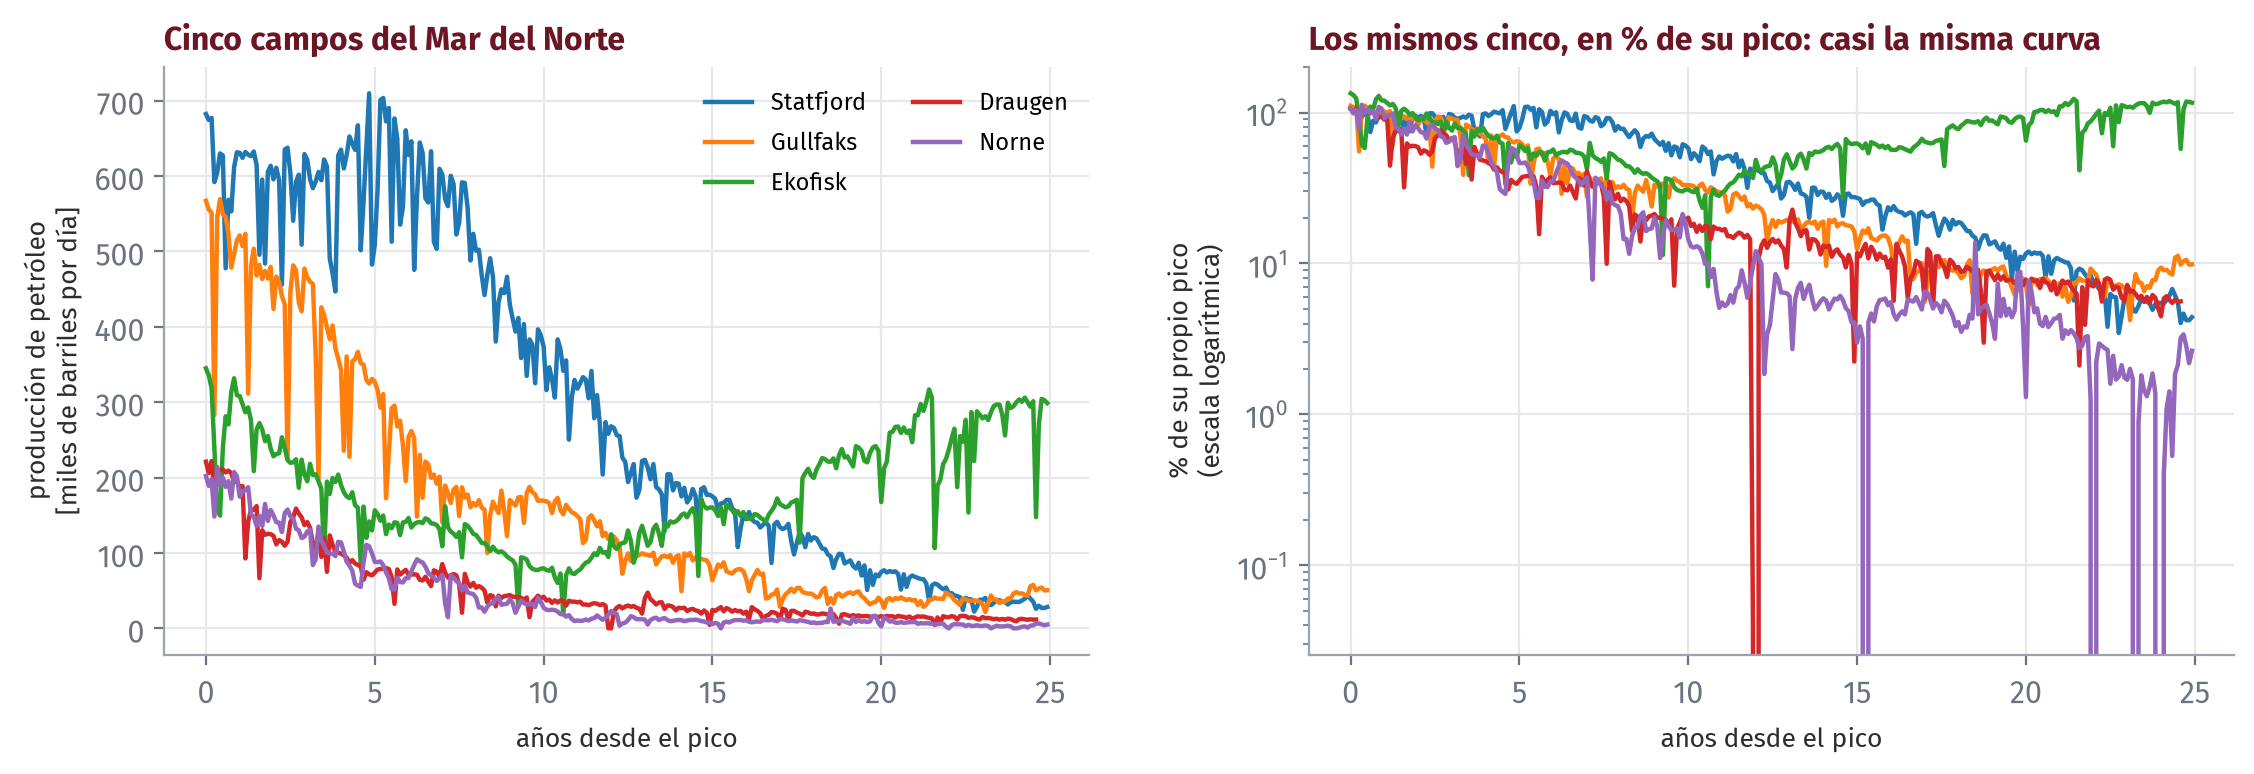
\includegraphics[height=0.44\textheight]{fig_que_es_declinacion.png}
  \end{center}
  \vspace{-2pt}
  {\footnotesize\color{textMuted}
  \begin{itemize}\setlength{\itemsep}{2pt}
    \item[{\color{arcaRed}\scriptsize\faArrowRight}]
      \textbf{Izquierda:} en barriles por día, cada campo es un mundo ---
      Statfjord arranca en 700 mil y Norne en 214 mil.
    \item[{\color{codeGreen}\scriptsize\faCheck}]
      \textbf{Derecha:} el mismo dato como \textbf{porcentaje de su propio
      pico} y en escala logarítmica. Y ahí aparece: es \emph{casi la misma
      curva}. Es el mismo truco de la Clase 2 --- comparar cada activo consigo
      mismo.
  \end{itemize}}
\end{frame}

\begin{frame}[shrink=8]{Alinear Desde el Pico (y Por Qué)}
  \vspace{-4pt}
  \begin{columns}[T]
    \begin{column}{0.50\textwidth}
      {\small\color{arcaDark}\bfseries\faQuestion\hspace{5pt}El problema}
      \vspace{4pt}
      {\footnotesize\color{textMuted}
      Ekofisk arrancó en 1971 y Grane en 2003. Si los ponemos en el mismo eje
      de calendario, no se parecen en nada: uno está muriendo cuando el otro
      todavía no nació.\\[6pt]
      Pero \textbf{la declinación no empieza en una fecha: empieza en el
      pico.} Antes del pico el campo todavía se está desarrollando ---
      se perforan pozos, se conecta capacidad.}
    \end{column}
    \begin{column}{0.46\textwidth}
      {\small\color{arcaDark}\bfseries\faCheck\hspace{5pt}Lo que hacemos}
      \vspace{4pt}
      {\footnotesize\color{textMuted}
      A cada campo le buscamos su mes de \textbf{producción máxima} y le
      ponemos ahí el cero de su reloj. De ahí en adelante, todos hablan el
      mismo idioma: \emph{«mes 37 después del pico»}.}
      \vspace{6pt}
      \begin{tcolorbox}[colback=arcaGray, colframe=arcaRed, boxrule=0pt, leftrule=3pt,
        arc=3pt, left=6pt, right=6pt, top=4pt, bottom=4pt]
        {\scriptsize\color{arcaRed}\bfseries\faExclamationTriangle\hspace{4pt}UN DETALLE QUE NO ES DETALLE}\\[3pt]
        {\scriptsize\color{textMuted}
         El pico lo buscamos sobre la producción \textbf{suavizada a seis
         meses}. Si no, un solo mes bueno --- un pozo nuevo que entró ---
         se lleva el pico a un lugar equivocado.}
      \end{tcolorbox}
    \end{column}
  \end{columns}
\end{frame}

\begin{frame}[shrink=6]{El Encargo, en una Figura}
  \vspace{-6pt}
  \begin{center}
    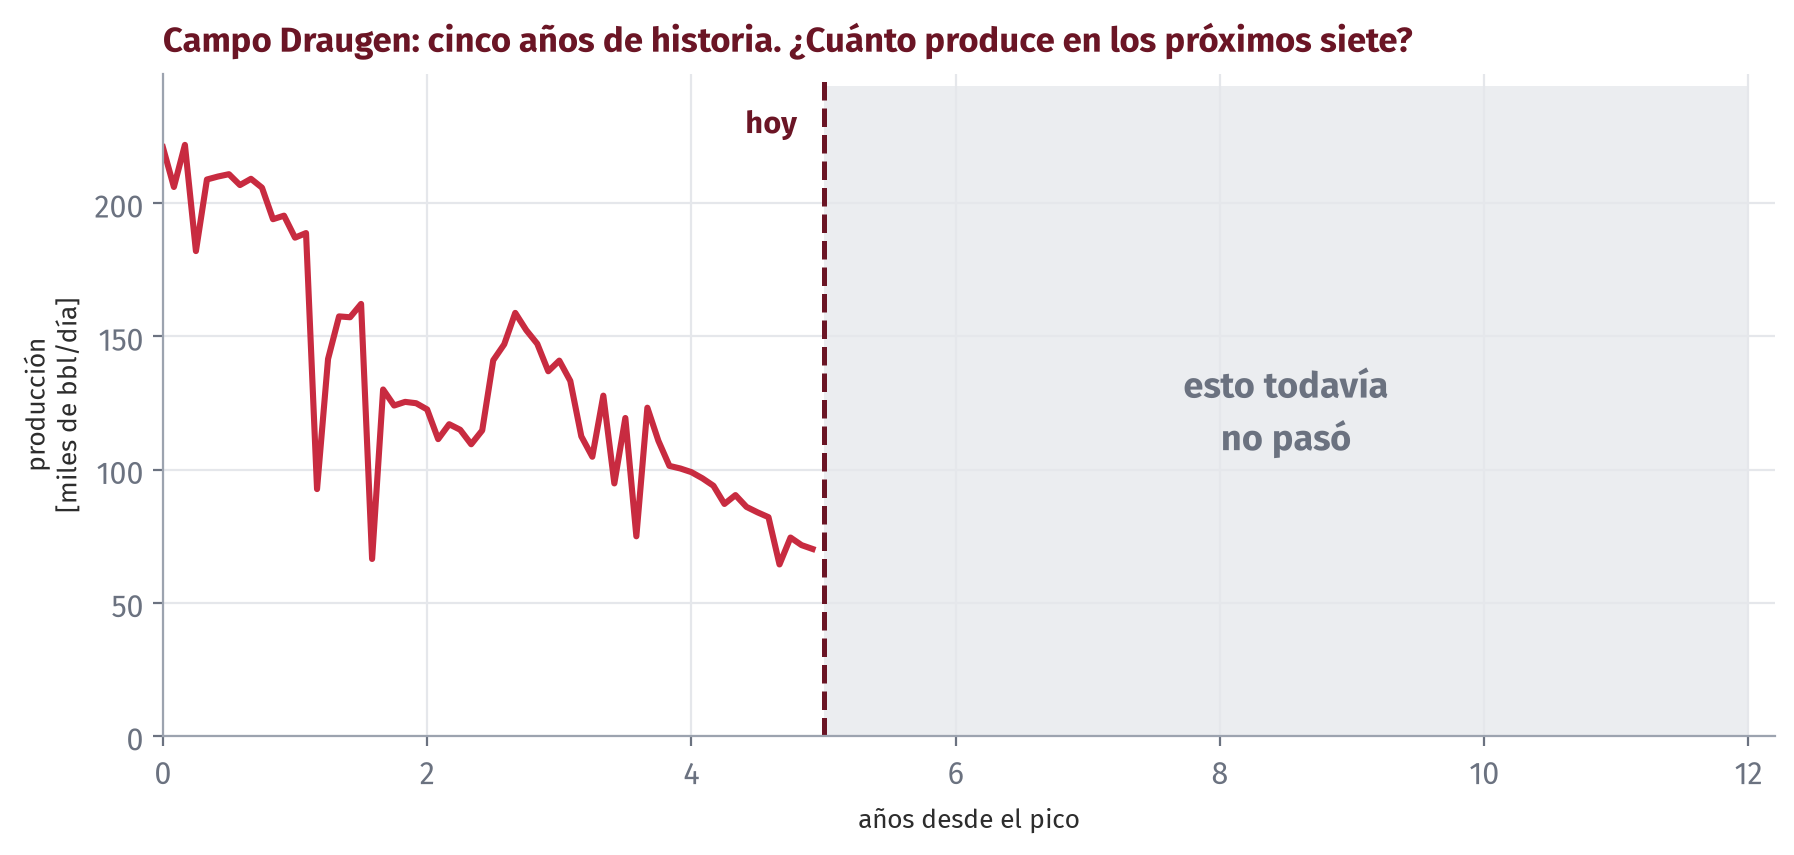
\includegraphics[height=0.56\textheight]{fig_el_encargo.png}
  \end{center}
  \vspace{-4pt}
  {\footnotesize\color{arcaDark}
   Todo lo que sigue es un intento de adivinar lo que hay debajo de esa
   mancha gris. Y al final la vamos a levantar.}
\end{frame}

\begin{frame}[fragile, shrink=22]{El Archivo}
  \vspace{-4pt}
  \begin{columns}[T]
    \begin{column}{0.56\textwidth}
      \begin{pyblock}
import pandas as pd

URL = ("https://raw.githubusercontent"
       ".com/cmosquerat/slb-diplomado"
       "/main/datos/"
       "campos_noruega_declinacion.csv")

d = pd.read_csv(URL)

print(d.campo.nunique(), "campos")
meses = d.groupby("campo").size()
print((meses / 12).describe().round(0))
      \end{pyblock}
    \end{column}
    \begin{column}{0.42\textwidth}
      \vspace{2pt}
      \begin{outputblock}
54 campos
16312 filas

count    54
mean     28
min      15
50%      25
max      49
      \end{outputblock}
      \vspace{4pt}
      {\footnotesize\color{textMuted}
      \begin{itemize}\setlength{\itemsep}{3pt}
        \item[{\color{arcaRed}\scriptsize\faDatabase}]
          \textbf{54 campos} del Mar del Norte noruego
        \item[{\color{arcaRed}\scriptsize\faClock}]
          Mediana de \textbf{25 años} después del pico
        \item[{\color{codeGreen}\scriptsize\faCheck}]
          El más viejo, \textbf{49 años}: Ekofisk, que sigue produciendo
      \end{itemize}}
    \end{column}
  \end{columns}
\end{frame}

\begin{frame}[shrink=10]{Las Variables, Una a Una}
  \vspace{-4pt}
  {\footnotesize
  \renewcommand{\arraystretch}{1.25}
  \begin{tabular}{@{}p{3.3cm}p{2.0cm}p{9.4cm}@{}}
    \toprule
    {\color{arcaDark}\bfseries columna} &
    {\color{arcaDark}\bfseries unidad} &
    {\color{arcaDark}\bfseries qué es} \\
    \midrule
    \texttt{campo} & --- & Nombre del campo. Es nuestra \textbf{unidad de análisis} \\
    \texttt{fecha} & --- & El mes de calendario \\
    \texttt{mes\_desde\_pico} & meses & \textbf{El reloj que importa}: 0 es el mes de máxima producción \\
    \texttt{dias} & días & Días que tuvo ese mes. Sirve para pasar de volumen a caudal \\
    \texttt{oil\_bpd} & bbl/día & \textbf{Lo que vamos a modelar}: producción media de petróleo \\
    \texttt{agua\_bpd} & bbl/día & Agua producida. Hoy no se usa --- es la Clase 4 \\
    \bottomrule
  \end{tabular}}
  \vspace{8pt}

  {\scriptsize\color{textMuted}\itshape
   El dato original del regulador noruego viene en \textbf{millones de metros
   cúbicos estándar por mes}. La conversión a barriles por día está en
   \texttt{preparar\_datos.py}, a la vista: un Sm³ son 6{,}2898 barriles, y se
   divide por los días del mes. Se dice porque su gerente piensa en barriles,
   no en metros cúbicos.}
\end{frame}

% ═════════════════════════════════════════════════════════════════════════════
\sectionframe{Arps, 1945}{La fórmula que la industria firma hace ochenta años --- y su defecto medible \\[6pt] \normalsize 35 -- 62 min}
% ═════════════════════════════════════════════════════════════════════════════

\begin{frame}[shrink=16]{Quién Fue Arps, y Qué Escribió}
  \vspace{-4pt}
  \begin{columns}[T]
    \begin{column}{0.50\textwidth}
      {\footnotesize\color{textMuted}
      \textbf{J. J. Arps}, ingeniero de petróleos, publicó en 1945 un trabajo
      donde hizo algo muy poco glamoroso: miró \textbf{muchísimas} curvas de
      producción reales y buscó una familia de fórmulas que las describiera.\\[6pt]
      No dedujo nada de la física del yacimiento. \textbf{Ajustó lo que veía.}
      Y ochenta años después esa familia sigue siendo la base de cómo se
      declaran las reservas en el mundo.}
      \vspace{7pt}
      \begin{tcolorbox}[colback=arcaGray, colframe=codeGreen, boxrule=0pt, leftrule=3pt,
        arc=3pt, left=6pt, right=6pt, top=4pt, bottom=4pt]
        {\scriptsize\color{codeGreen}\bfseries\faCheck\hspace{4pt}POR QUÉ SOBREVIVIÓ}\\[3pt]
        {\scriptsize\color{textMuted}
         Porque tiene \textbf{pocos parámetros}, se ajusta con poca historia,
         y cada parámetro significa algo que un ingeniero puede discutir en
         una reunión.}
      \end{tcolorbox}
    \end{column}
    \begin{column}{0.46\textwidth}
      {\small\color{arcaDark}\bfseries\faSitemap\hspace{5pt}La familia, en una lámina}
      \vspace{5pt}
      {\footnotesize\color{textMuted}
      Una sola fórmula con un botón, \textbf{b}, que la cambia de forma:
      \vspace{5pt}
      \begin{itemize}\setlength{\itemsep}{5pt}
        \item[{\color{arcaRed}\scriptsize\faCircle}]
          \textbf{b = 0} $\rightarrow$ \textbf{exponencial}.
          La recta de la Clase 1
        \item[{\color{codeBlue}\scriptsize\faCircle}]
          \textbf{0 < b < 1} $\rightarrow$ \textbf{hiperbólica}.
          Lo que se ve casi siempre
        \item[{\color{codeGreen}\scriptsize\faCircle}]
          \textbf{b = 1} $\rightarrow$ \textbf{armónica}.
          La cola más gorda posible
      \end{itemize}}
      \vspace{6pt}
      {\scriptsize\color{arcaDark}\itshape
        Vamos a empezar por la de la Clase 1, medirle el defecto,
        y recién ahí ganarnos el derecho a la siguiente.}
    \end{column}
  \end{columns}
\end{frame}

\begin{frame}[shrink=6]{La Exponencial: la Recta de la Clase 1, Con Nombre}
  \vspace{-6pt}
  \begin{center}
    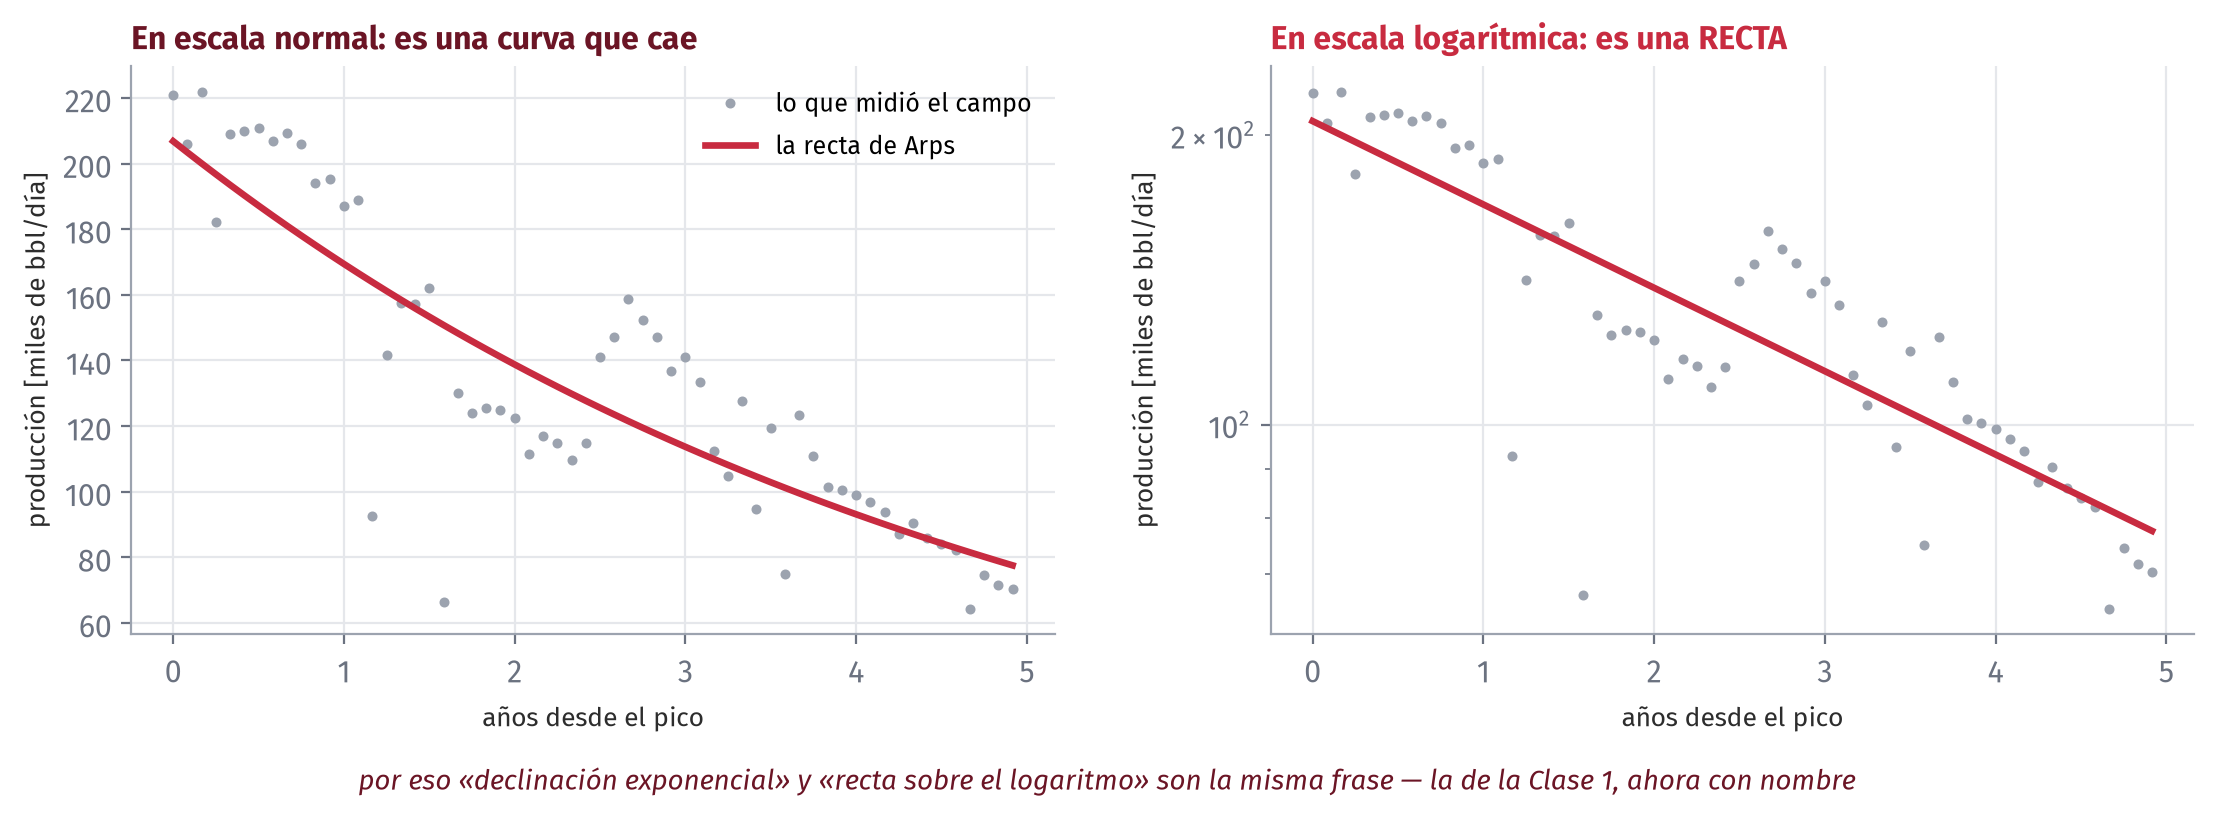
\includegraphics[height=0.56\textheight]{fig_que_es_arps.png}
  \end{center}
  \vspace{-2pt}
  {\footnotesize\color{textMuted}
   Si cada mes se pierde el \emph{mismo porcentaje} --- no la misma cantidad,
   el mismo porcentaje --- entonces al dibujar el logaritmo sale una recta.
   Eso, y solo eso, es la declinación exponencial.}
\end{frame}

\begin{frame}[shrink=4]{Doblando el Eje de a Poco}
  \vspace{-10pt}
  \begin{center}
    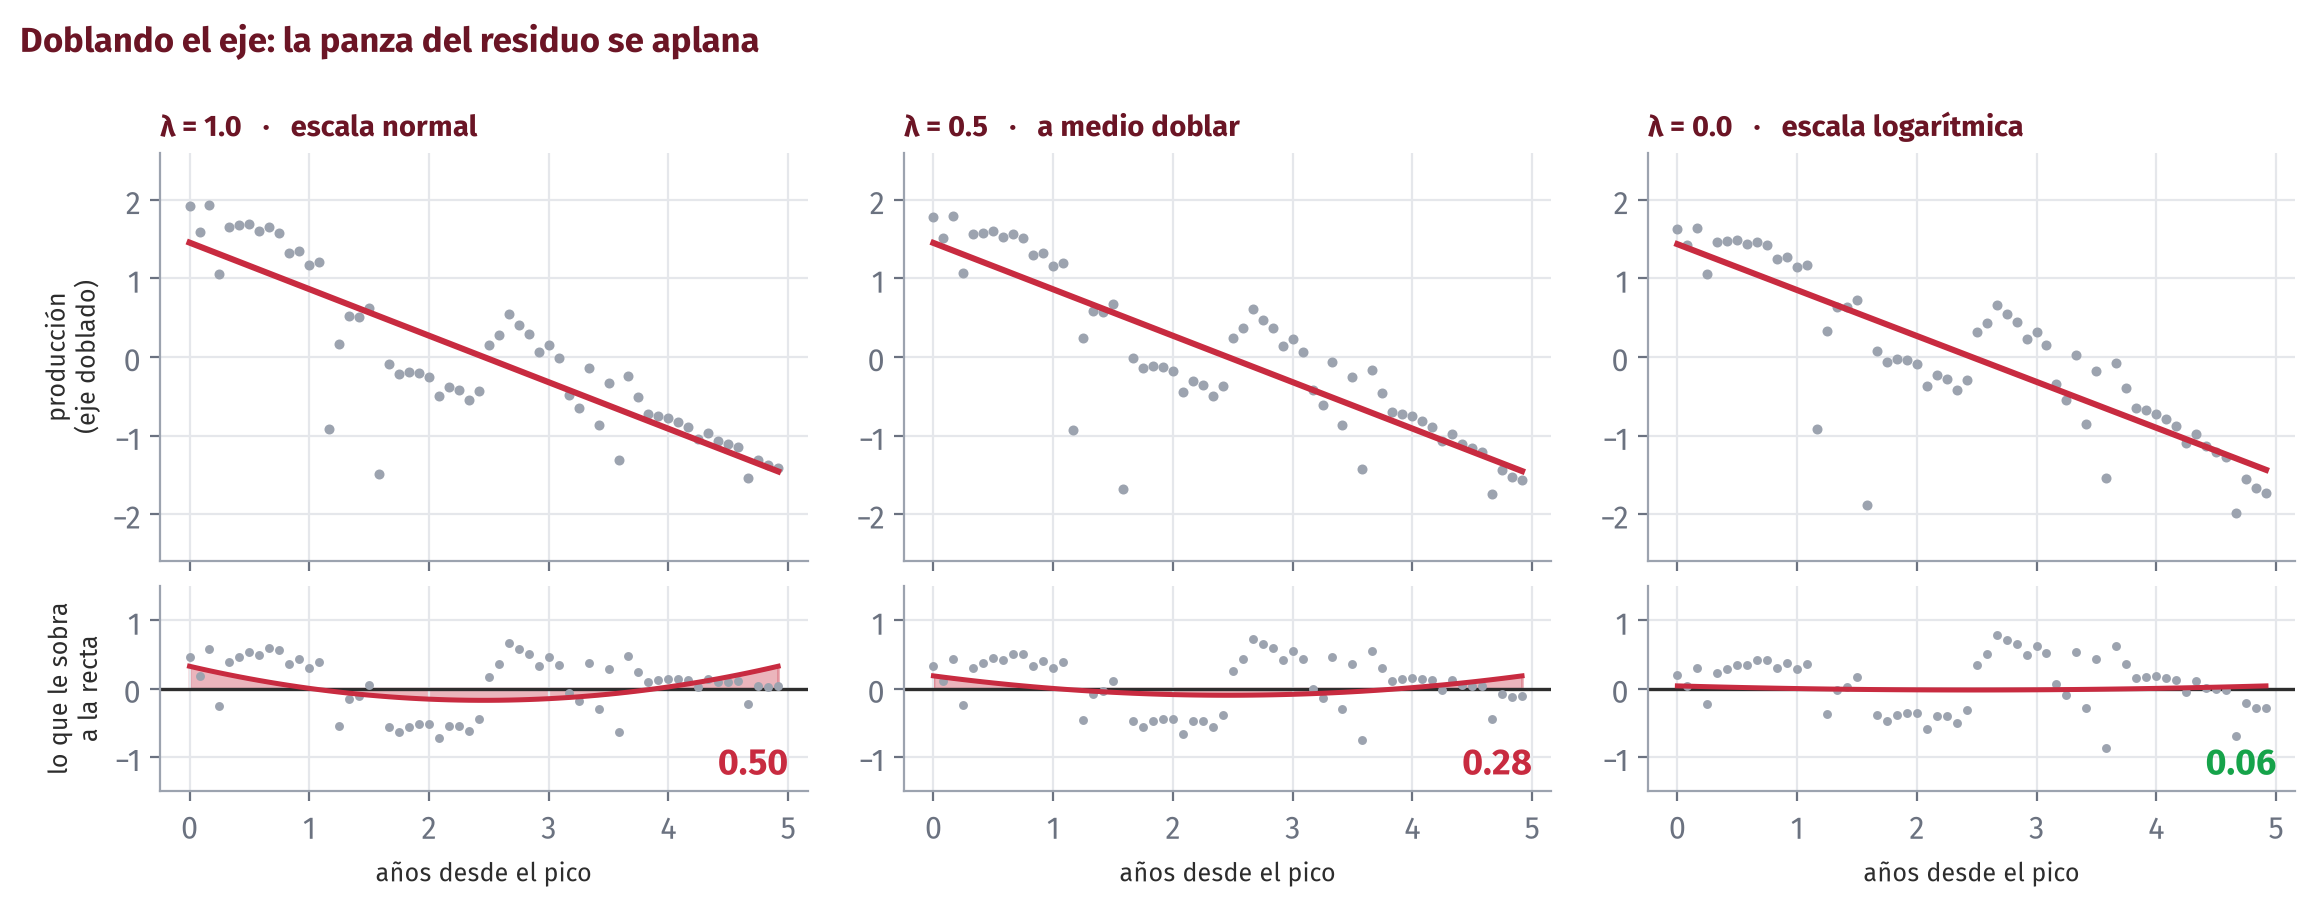
\includegraphics[height=0.60\textheight]{fig_doblar.png}
  \end{center}
  \vspace{-6pt}
  {\footnotesize\color{arcaDark}
   Miren \textbf{la fila de abajo}. Sin doblar el eje, al residuo le queda
   \textbf{panza}; doblado, no le queda forma --- y cuando no le queda forma,
   la recta es el modelo correcto.}
\end{frame}

\begin{frame}[shrink=8]{Pero No Siempre Alcanza con Doblar el Eje}
  \vspace{-4pt}
  {\small\color{arcaDark}\bfseries
   Draugen quedó precioso. La regla de la casa es no creerle a un campo.}
  \vspace{10pt}
  \begin{columns}[T]
    \begin{column}{0.42\textwidth}
      \begin{tcolorbox}[colback=arcaGray, colframe=arcaRed, boxrule=0pt, leftrule=3pt,
        arc=3pt, left=6pt, right=6pt, top=7pt, bottom=7pt]
        \centering
        {\scriptsize\color{textMuted}EL LOGARITMO ENDEREZA EN}\\[5pt]
        {\LARGE\color{arcaRed}\bfseries 33 de 53}\\[5pt]
        {\scriptsize\color{textMuted}campos --- el 62 \%}
      \end{tcolorbox}
    \end{column}
    \begin{column}{0.54\textwidth}
      {\footnotesize\color{textMuted}
      En el tercio restante, doblar el eje \textbf{no alcanza}: la curva sigue
      arqueada aunque la miremos en logaritmo.\\[7pt]
      Ese tercio son los campos con \textbf{cola} --- los que se resisten a
      morir. Y son exactamente los que la exponencial va a subestimar.}
      \vspace{7pt}
      {\footnotesize\color{arcaDark}\itshape
       Anótenlo: es la razón de que exista la segunda mitad de esta clase.}
    \end{column}
  \end{columns}
  \vspace{9pt}
  {\scriptsize\color{textMuted}\itshape
   En el cuaderno esto se ve \textbf{en movimiento}: una animación dobla el eje
   de forma continua y muestra la panza del residuo aplanándose, cuadro a cuadro.}
\end{frame}

\begin{frame}[shrink=8]{Qué es D, y Por Qué se Discute en las Reuniones}
  \vspace{-4pt}
  \begin{columns}[T]
    \begin{column}{0.50\textwidth}
      {\footnotesize\color{textMuted}
      La pendiente de esa recta tiene nombre: \textbf{D}, la \emph{tasa de
      declinación}. Se dice en \textbf{porcentaje por año}.\\[6pt]
      \textit{«Este campo declina al 18 \% anual»} quiere decir: dentro de un
      año va a estar produciendo un 18 \% menos que hoy. Y al año siguiente,
      un 18 \% menos que eso.}
      \vspace{6pt}
      {\footnotesize\color{arcaDark}
       En nuestros 54 campos la mediana es \textbf{18 \% al año}. Es
       un número perfectamente típico para un campo offshore maduro.}
    \end{column}
    \begin{column}{0.46\textwidth}
      \begin{tcolorbox}[colback=arcaGray, colframe=arcaRed, boxrule=0pt, leftrule=3pt,
        arc=3pt, left=6pt, right=6pt, top=5pt, bottom=5pt]
        {\scriptsize\color{arcaRed}\bfseries\faExclamationTriangle\hspace{4pt}CUIDADO CON EL PORCENTAJE}\\[4pt]
        {\scriptsize\color{textMuted}
         Perder el 18 \% cada año \textbf{no} es perder todo en cinco años y
         medio.\\[4pt]
         Es como el interés compuesto, pero al revés: siempre queda algo.
         A los 5 años queda el 37 \%; a los 10, el 14 \%; a los 20,
         el 2 \%. Nunca llega exactamente a cero.\\[4pt]
         Esa \textbf{cola} que nunca se apaga es de lo que vamos a discutir
         el resto de la clase.}
      \end{tcolorbox}
    \end{column}
  \end{columns}
\end{frame}

\begin{frame}[fragile, shrink=20]{La Exponencial, en Código}
  \vspace{-4pt}
  \begin{columns}[T]
    \begin{column}{0.58\textwidth}
      \begin{pyblock}
q = campos["DRAUGEN"]     # bbl/dia
y = q.iloc[:60].values    # 5 anios
t = np.arange(60)         # 0 ... 59

# una RECTA sobre el LOGARITMO
b = np.polyfit(t, np.log(y), 1)
D = 100 * (1 - np.exp(b[0] * 12))
print("declina", round(D), "% al anio")

m = np.arange(144)        # 12 anios
acum = np.exp(np.polyval(b, m)).sum()
print(round(acum*30.4/1e6, 1), "MMbbl")
      \end{pyblock}
    \end{column}
    \begin{column}{0.40\textwidth}
      \vspace{2pt}
      \begin{outputblock}
declina 18 % al anio
346.6 MMbbl
      \end{outputblock}
      \vspace{6pt}
      {\footnotesize\color{textMuted}
      Línea por línea:
      \vspace{4pt}
      \begin{itemize}\setlength{\itemsep}{4pt}
        \item[{\color{arcaRed}\scriptsize\faArrowRight}]
          \texttt{np.log(y)} $\rightarrow$ doblamos el eje para que
          la curva se vuelva recta
        \item[{\color{arcaRed}\scriptsize\faArrowRight}]
          \texttt{polyfit(\dots, 1)} $\rightarrow$ la recta que mejor pasa
          por esos puntos. Es el \texttt{LinearRegression} del M3·C1,
          en su versión más corta
        \item[{\color{arcaRed}\scriptsize\faArrowRight}]
          \texttt{np.exp(\dots)} $\rightarrow$ desdoblamos el eje para
          volver a barriles
      \end{itemize}}
    \end{column}
  \end{columns}
\end{frame}

\begin{frame}[shrink=6]{Ahora Destapamos: ¿Cuánto se Equivocó?}
  \vspace{-6pt}
  \begin{center}
    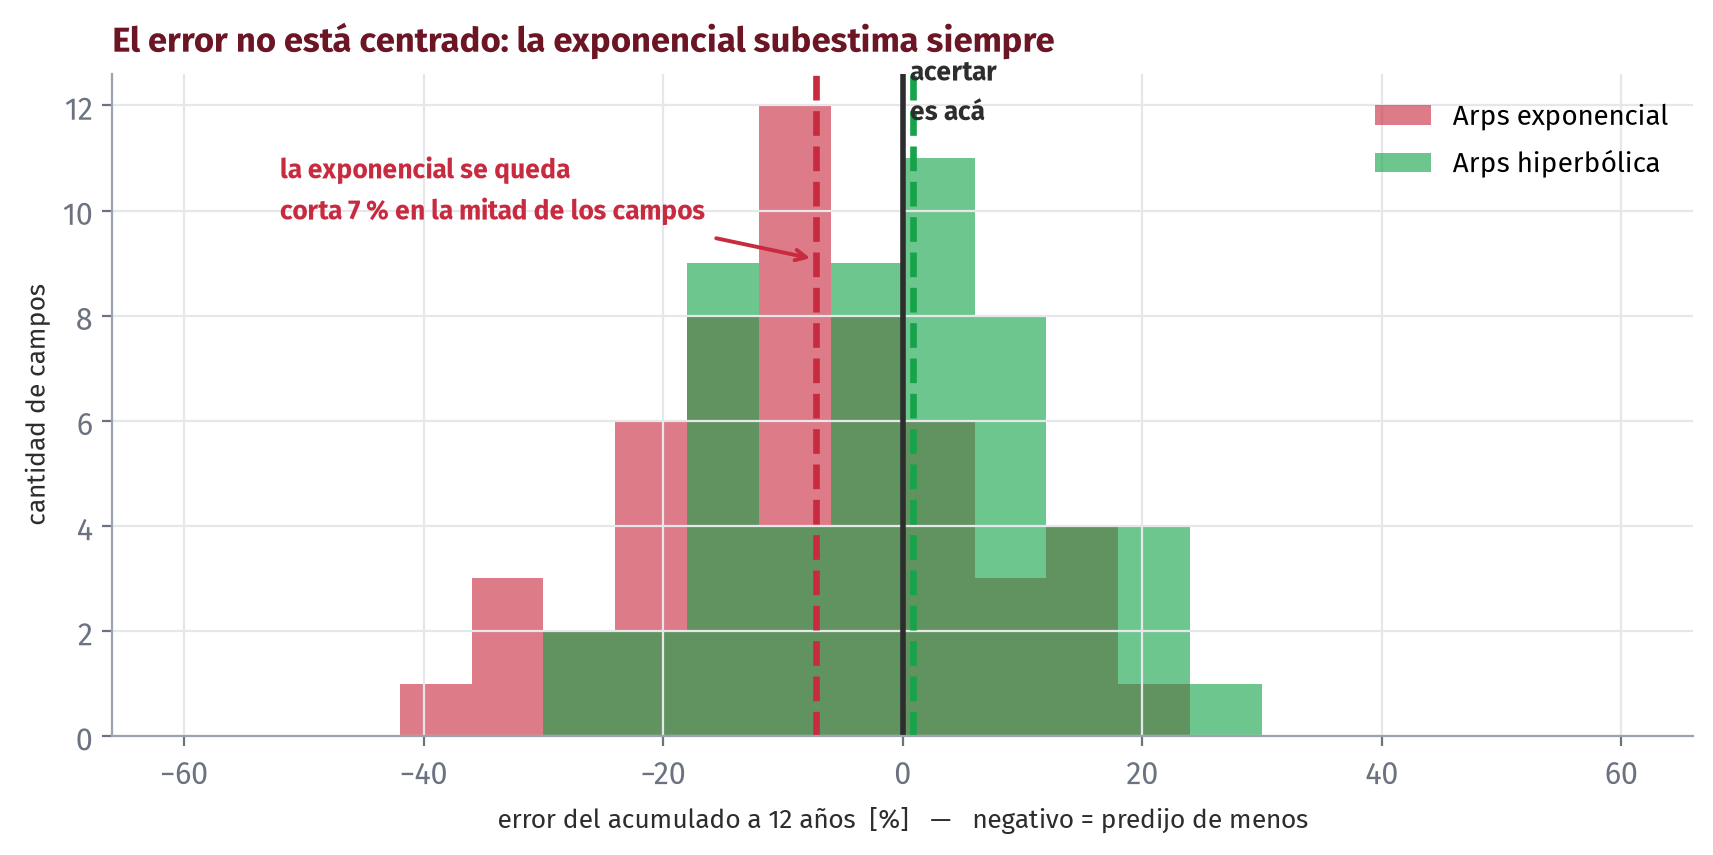
\includegraphics[height=0.50\textheight]{fig_sesgo.png}
  \end{center}
  \vspace{-2pt}
  {\footnotesize\color{arcaDark}
   Si el método fuera solo \emph{impreciso}, el histograma estaría centrado en
   cero y repartido a los dos lados. \textbf{No lo está.} Está corrido a la
   izquierda: la exponencial no se equivoca al azar, se equivoca
   \textbf{siempre para el mismo lado}.}
\end{frame}

\begin{frame}[shrink=16]{Error y Sesgo No Son lo Mismo}
  \vspace{-4pt}
  {\small\color{arcaDark}\bfseries
   Esta distinción vale para todo lo que hagan con datos, no solo para
   curvas de declinación.}
  \vspace{9pt}
  \begin{columns}[T]
    \begin{column}{0.47\textwidth}
      \begin{tcolorbox}[colback=arcaGray, colframe=codeBlue, boxrule=0pt, leftrule=3pt,
        arc=3pt, left=6pt, right=6pt, top=5pt, bottom=5pt]
        {\scriptsize\color{codeBlue}\bfseries\faBullseye\hspace{4pt}ERROR (imprecisión)}\\[4pt]
        {\scriptsize\color{textMuted}
         Le pego a veces arriba y a veces abajo. Molesta, pero
         \textbf{se compensa}: si tengo veinte campos, los de más y los de
         menos se cancelan y la cartera queda bien.}
      \end{tcolorbox}
    \end{column}
    \begin{column}{0.47\textwidth}
      \begin{tcolorbox}[colback=arcaGray, colframe=arcaRed, boxrule=0pt, leftrule=3pt,
        arc=3pt, left=6pt, right=6pt, top=5pt, bottom=5pt]
        {\scriptsize\color{arcaRed}\bfseries\faExclamationTriangle\hspace{4pt}SESGO (error sistemático)}\\[4pt]
        {\scriptsize\color{textMuted}
         Le pego \textbf{siempre para el mismo lado}. No se compensa nunca:
         con veinte campos me equivoco veinte veces en la misma dirección, y
         la cartera entera queda mal.}
      \end{tcolorbox}
    \end{column}
  \end{columns}
  \vspace{9pt}
  \begin{tcolorbox}[colback=arcaGray, colframe=arcaDark, boxrule=0pt, leftrule=3pt,
    arc=3pt, left=8pt, right=8pt, top=6pt, bottom=6pt]
    {\footnotesize\color{textMuted}
     La exponencial tiene un sesgo de \textbf{--7 \%}. En la mitad de los
     campos declara \emph{de menos}. Para reservas eso suena conservador y
     prudente\dots\ pero significa que sistemáticamente se subvalúan activos,
     y se abandonan campos antes de tiempo.\\[5pt]
     {\color{arcaDark}\bfseries Y tiene una explicación física, no estadística:
      la exponencial no cree en la cola.}}
  \end{tcolorbox}
\end{frame}

\begin{frame}[shrink=6]{La Hiperbólica: Qué es b}
  \vspace{-6pt}
  \begin{center}
    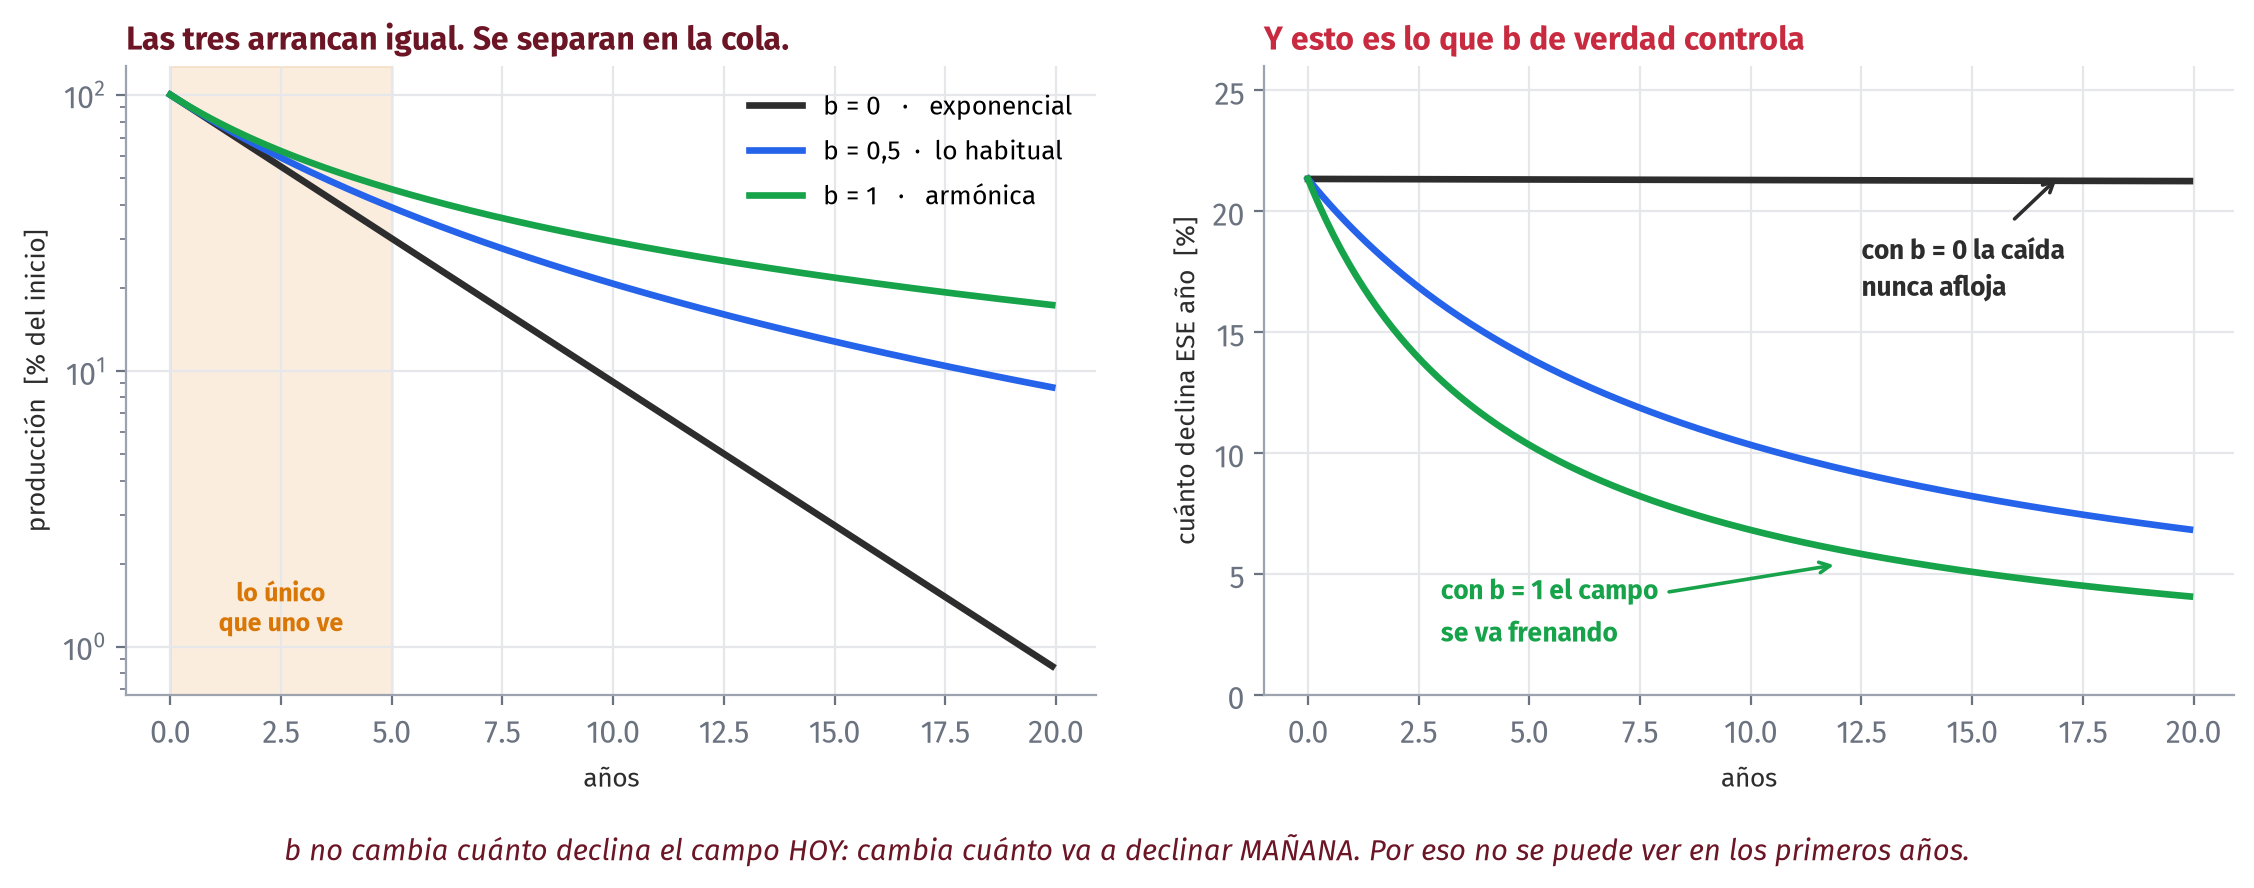
\includegraphics[height=0.56\textheight]{fig_que_es_b.png}
  \end{center}
  \vspace{-2pt}
  {\footnotesize\color{textMuted}
   \textbf{b} mide cuánto se \emph{frena} la declinación con el tiempo. Con
   b = 0 el campo pierde el mismo porcentaje para siempre. Con b > 0 el
   porcentaje que pierde va bajando: el campo se resiste a morir.}
\end{frame}

\begin{frame}[shrink=8]{Por Qué Existe la Cola (y no es un truco matemático)}
  \vspace{-4pt}
  \begin{columns}[T]
    \begin{column}{0.51\textwidth}
      {\footnotesize\color{textMuted}
      Un campo no es un tanque homogéneo. Tiene zonas buenas, muy permeables,
      que se drenan rápido; y zonas apretadas que entregan lento.\\[6pt]
      Al principio produce sobre todo lo fácil, y la caída es rápida.
      Cuando lo fácil se agotó, lo que queda es lo lento --- y \textbf{lo
      lento cae despacio}.\\[6pt]
      Por eso la declinación se \textbf{frena}. Y por eso b es casi siempre
      mayor que cero en un campo real.}
    \end{column}
    \begin{column}{0.45\textwidth}
      \begin{tcolorbox}[colback=arcaGray, colframe=arcaDark, boxrule=0pt, leftrule=3pt,
        arc=3pt, left=6pt, right=6pt, top=5pt, bottom=5pt]
        {\scriptsize\color{arcaDark}\bfseries\faChartLine\hspace{4pt}LO QUE ENCONTRAMOS}\\[4pt]
        {\scriptsize\color{textMuted}
         Ajustamos b libremente en los 54 campos:\\[4pt]
         mediana \textbf{b = 0{,}07}\\
         y \textbf{26 de 54} campos con b > 0{,}1.\\[5pt]
         O sea: en la mitad la hiperbólica eligió sola volverse casi
         exponencial. En la otra mitad, no --- y ahí es donde importó.}
      \end{tcolorbox}
      \vspace{5pt}
      {\scriptsize\color{arcaRed}\bfseries\itshape
        Ojo con b > 1: matemáticamente el acumulado se vuelve infinito.
        Si el ajuste les da eso, está mal.}
    \end{column}
  \end{columns}
\end{frame}

\begin{frame}[fragile, shrink=20]{La Hiperbólica, en Código}
  \vspace{-4pt}
  \begin{columns}[T]
    \begin{column}{0.58\textwidth}
      \begin{pyblock}
from scipy.optimize import curve_fit

# la formula de Arps, de 1945
def hiperbolica(t, qi, Di, b):
    return qi / (1+b*Di*t) ** (1/b)

# bounds = barandas: b entre 0 y 2
p, _ = curve_fit(hiperbolica, t, y,
    p0=[y[0], 0.02, 0.5],
    bounds=([0, 1e-6, 1e-3],
            [np.inf, 1.0, 2.0]))
print("b =", round(p[2], 2))
      \end{pyblock}
    \end{column}
    \begin{column}{0.40\textwidth}
      \vspace{2pt}
      \begin{outputblock}
b = 0.91
      \end{outputblock}
      \vspace{6pt}
      {\footnotesize\color{textMuted}
      \begin{itemize}\setlength{\itemsep}{4pt}
        \item[{\color{arcaRed}\scriptsize\faArrowRight}]
          Acá ya no alcanza una recta: la fórmula no es lineal, así que
          hace falta un buscador
        \item[{\color{arcaRed}\scriptsize\faArrowRight}]
          \texttt{bounds} le pone \textbf{barandas}: b entre 0 y 2.
          Sin eso, el ajuste se va a valores sin sentido físico
        \item[{\color{codeGreen}\scriptsize\faCheck}]
          Draugen dio \textbf{b = 0{,}91}: un campo con mucha cola
      \end{itemize}}
    \end{column}
  \end{columns}
\end{frame}

\begin{frame}[shrink=6]{Las Dos Curvas, y lo que Pasó}
  \vspace{-6pt}
  \begin{center}
    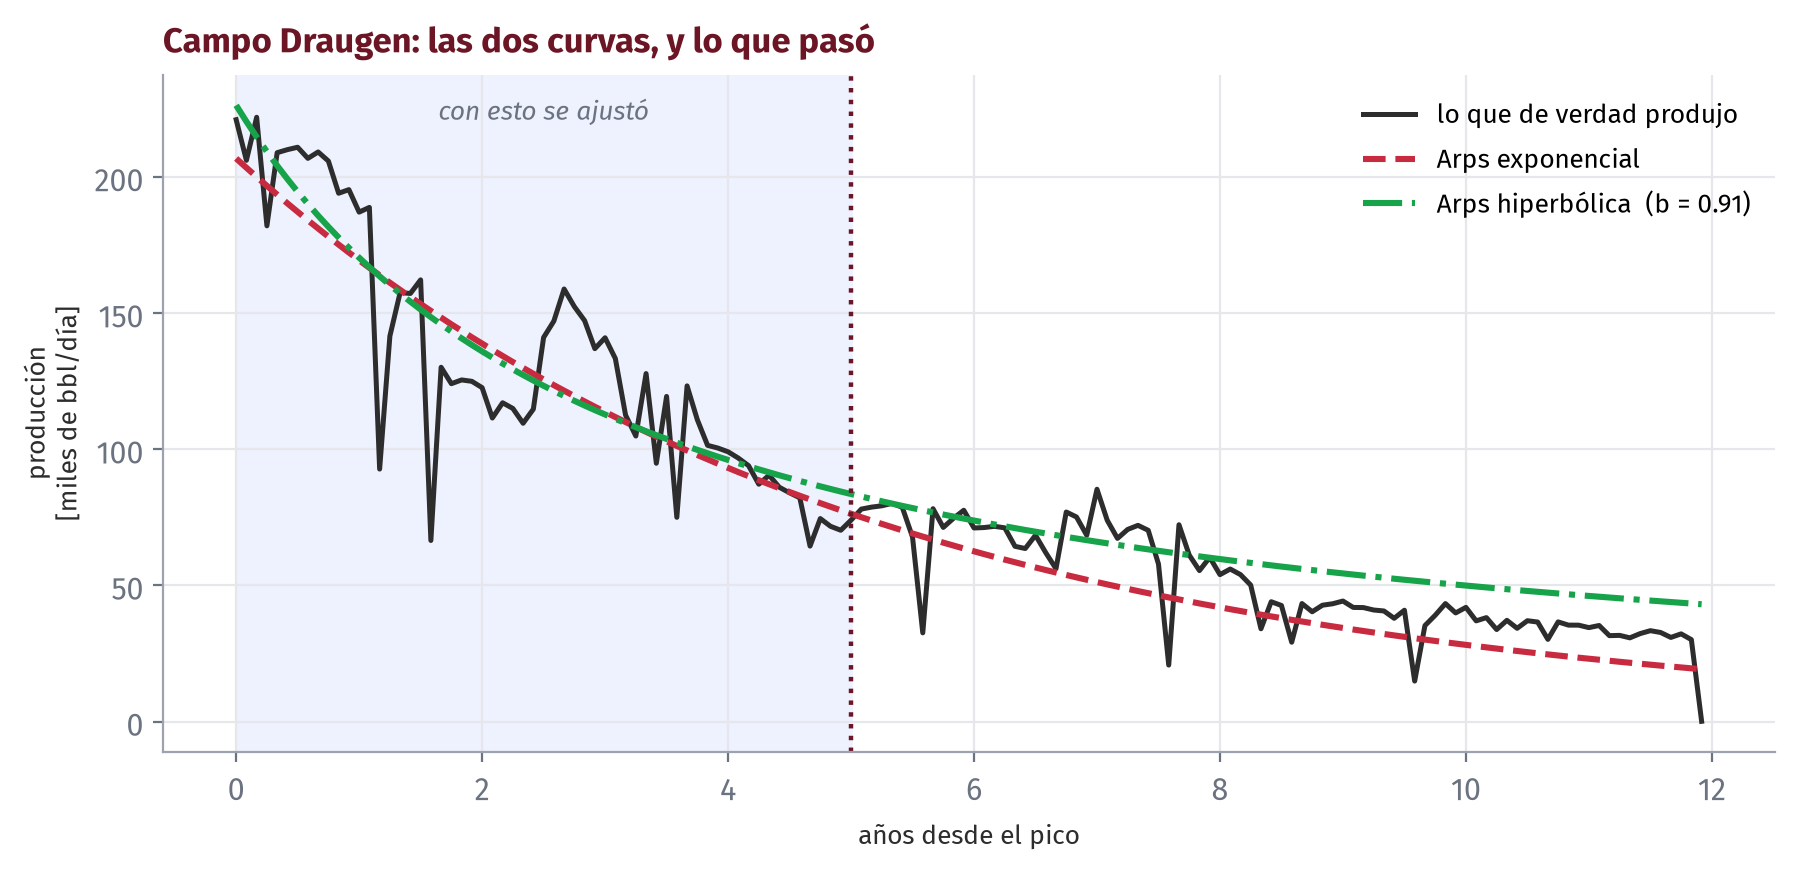
\includegraphics[height=0.54\textheight]{fig_ajuste_comparado.png}
  \end{center}
  \vspace{-4pt}
  {\footnotesize\color{arcaDark}
   Las dos se ajustan igual de bien a la zona azul --- que es todo lo que
   se ve al firmar. Se separan justo donde nadie puede mirar.}
\end{frame}

% ═════════════════════════════════════════════════════════════════════════════
\sectionframe{Y Ahora, en Dólares}{Un campo no produce hasta cero: produce hasta que deja de pagar \\[6pt] \normalsize 62 -- 80 min}
% ═════════════════════════════════════════════════════════════════════════════

\begin{frame}[shrink=16]{El Campo No Produce Hasta Cero}
  \vspace{-4pt}
  {\small\color{arcaDark}\bfseries
   Todo lo que hicimos hasta acá pronostica barriles. Pero nadie produce
   barriles que cuesten más de lo que valen.}
  \vspace{8pt}
  \begin{columns}[T]
    \begin{column}{0.50\textwidth}
      {\footnotesize\color{textMuted}
      Un campo tiene dos tipos de costo:
      \vspace{5pt}
      \begin{itemize}\setlength{\itemsep}{5pt}
        \item[{\color{arcaRed}\scriptsize\faArrowRight}]
          \textbf{Variable} --- lo que cuesta sacar cada barril: energía,
          químicos, tratar el agua. Se paga por barril.
        \item[{\color{arcaRed}\scriptsize\faArrowRight}]
          \textbf{Fijo} --- lo que cuesta tener el campo \emph{abierto}:
          la plataforma, la gente, el mantenimiento, los seguros. Se paga
          igual, produzca mucho o poco.
      \end{itemize}}
      \vspace{7pt}
      {\footnotesize\color{arcaDark}
       Cuando la producción baja tanto que \textbf{ya no alcanza para pagar
       el costo fijo}, el campo pierde plata todos los meses. Ese caudal se
       llama \textbf{límite económico}.}
    \end{column}
    \begin{column}{0.46\textwidth}
      \begin{tcolorbox}[colback=arcaGray, colframe=arcaDark, boxrule=0pt, leftrule=3pt,
        arc=3pt, left=6pt, right=6pt, top=5pt, bottom=5pt]
        {\scriptsize\color{arcaDark}\bfseries\faCalculator\hspace{4pt}LA CUENTA, COMPLETA}\\[5pt]
        {\scriptsize\color{textMuted}
        \[ q_{\text{límite}}=\frac{\text{costo fijo del mes}}
                                  {(\text{precio}-\text{costo variable})\times\text{días}} \]
        \vspace{-4pt}
        Con los supuestos de esta clase:\\[3pt]
        precio \textbf{70} -- opex \textbf{15} $=$ margen \textbf{55 USD/bbl}\\
        costo fijo \textbf{8 millones de USD al mes}\\[4pt]
        {\color{arcaRed}\bfseries $q_{\text{límite}}\approx 4\,785$ bbl/día}}
      \end{tcolorbox}
      \vspace{5pt}
      {\scriptsize\color{arcaDark}\itshape
        Esos tres números los pone finanzas, no el ingeniero de yacimientos.
        Van a la vista justamente para que se puedan discutir.}
    \end{column}
  \end{columns}
\end{frame}

\begin{frame}[shrink=6]{La Curva Elegida Decide el Año de Cierre}
  \vspace{-6pt}
  \begin{center}
    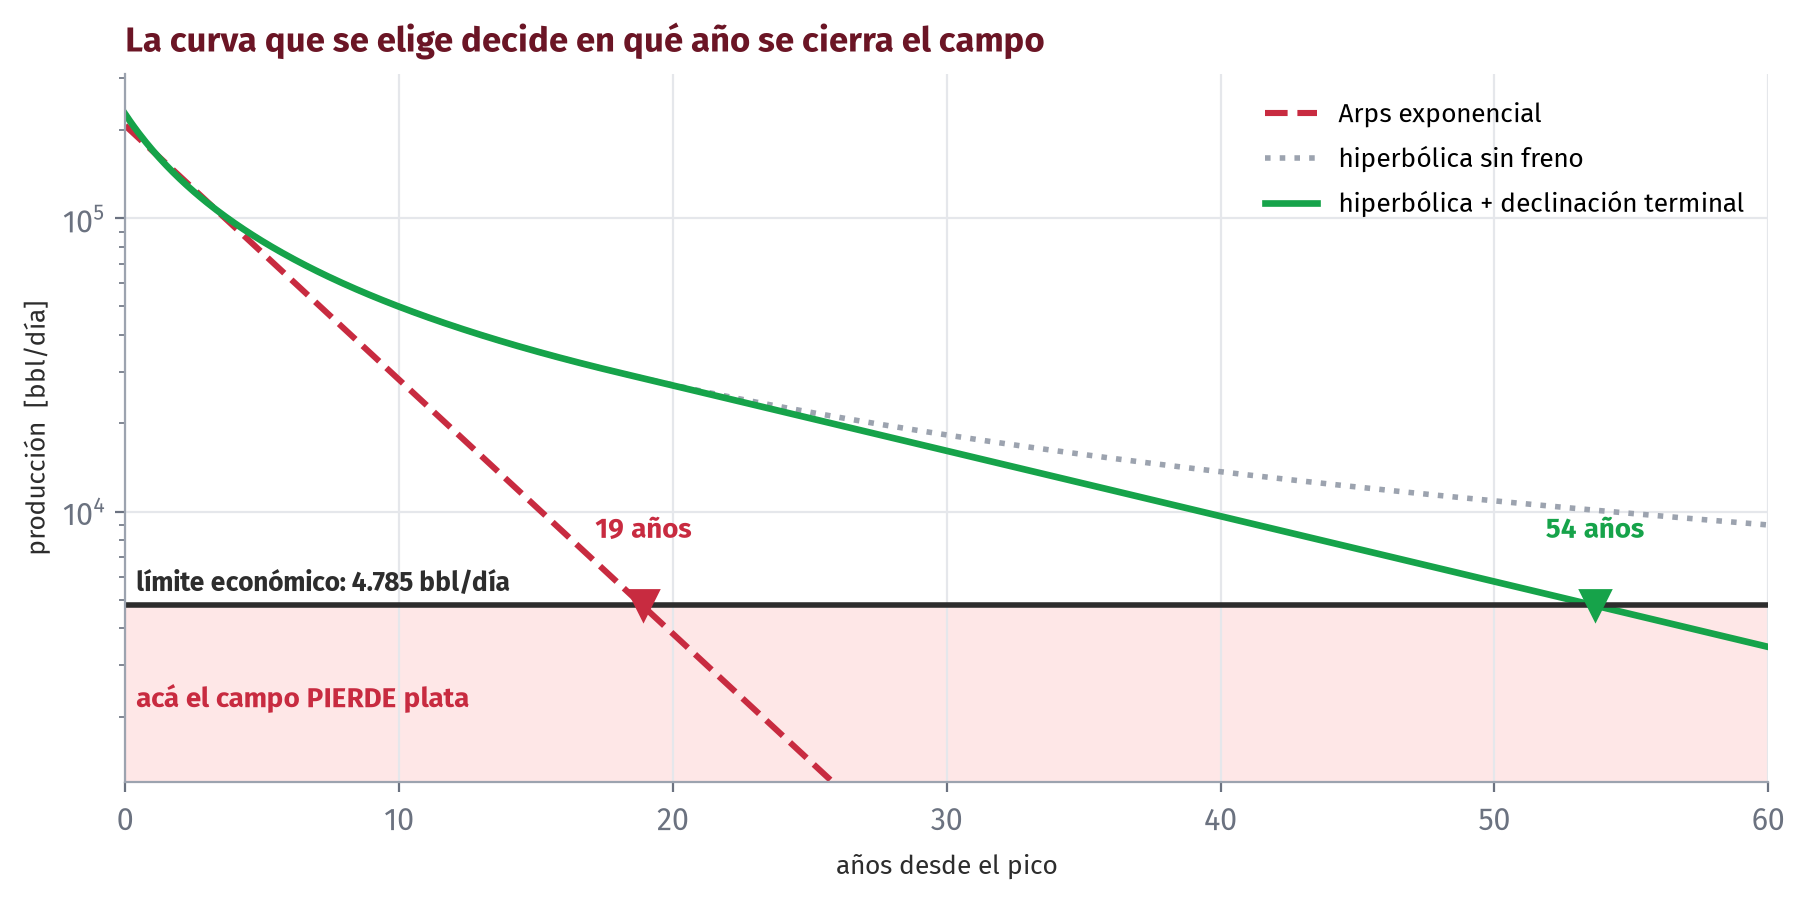
\includegraphics[height=0.54\textheight]{fig_limite_economico.png}
  \end{center}
  \vspace{-4pt}
  {\footnotesize\color{arcaDark}
   Mismo campo, mismos cinco años de historia. Según la exponencial cierra a
   los \textbf{19 años}; con la hiperbólica frenada, a los \textbf{54}.
   No es un matiz técnico: es cuándo se despide a la gente.}
\end{frame}

\begin{frame}[shrink=16]{La Trampa de la Cola: Campos Inmortales}
  \vspace{-4pt}
  {\small\color{arcaDark}\bfseries
   Y acá aparece el defecto de la hiperbólica, que es tan grave como el de
   la exponencial --- solo que al revés.}
  \vspace{8pt}
  \begin{columns}[T]
    \begin{column}{0.48\textwidth}
      \begin{tcolorbox}[colback=arcaGray, colframe=arcaRed, boxrule=0pt, leftrule=3pt,
        arc=3pt, left=6pt, right=6pt, top=5pt, bottom=5pt]
        {\scriptsize\color{arcaRed}\bfseries\faExclamationTriangle\hspace{4pt}EL PROBLEMA, MEDIDO}\\[4pt]
        {\scriptsize\color{textMuted}
         Con b cerca de 1, la declinación se frena tanto que la curva
         \textbf{nunca} cruza el límite económico.\\[5pt]
         En nuestros campos eso pasa en {\color{arcaRed}\bfseries 12 de 54}.
         El modelo está diciendo, literalmente, que el campo
         \textbf{no se muere nunca}.\\[5pt]
         Draugen es uno de ellos.}
      \end{tcolorbox}
    \end{column}
    \begin{column}{0.48\textwidth}
      \begin{tcolorbox}[colback=arcaGray, colframe=codeGreen, boxrule=0pt, leftrule=3pt,
        arc=3pt, left=6pt, right=6pt, top=5pt, bottom=5pt]
        {\scriptsize\color{codeGreen}\bfseries\faCheck\hspace{4pt}LA CORRECCIÓN ESTÁNDAR}\\[4pt]
        {\scriptsize\color{textMuted}
         Se le pone un \textbf{piso a la declinación}: cuando la hiperbólica
         cae por debajo de un mínimo --- acá, \textbf{5 \% al año} --- se
         cambia a exponencial y de ahí en adelante decae parejo.\\[5pt]
         Se llama \textbf{declinación terminal}, y con ella los campos
         inmortales bajan de 12 a {\color{codeGreen}\bfseries 4 de 54}.}
      \end{tcolorbox}
    \end{column}
  \end{columns}
  \vspace{8pt}
  {\footnotesize\color{arcaDark}\itshape
   Ninguna de las dos curvas es «la buena». La exponencial se queda corta,
   la hiperbólica se pasa de largo, y el trabajo del ingeniero es saber
   \textbf{dónde ponerle el freno} --- porque la fórmula sola no lo sabe.}
\end{frame}

\begin{frame}[shrink=6]{El Sesgo del 7 \%, en el Idioma de Gerencia}
  \vspace{-6pt}
  \begin{center}
    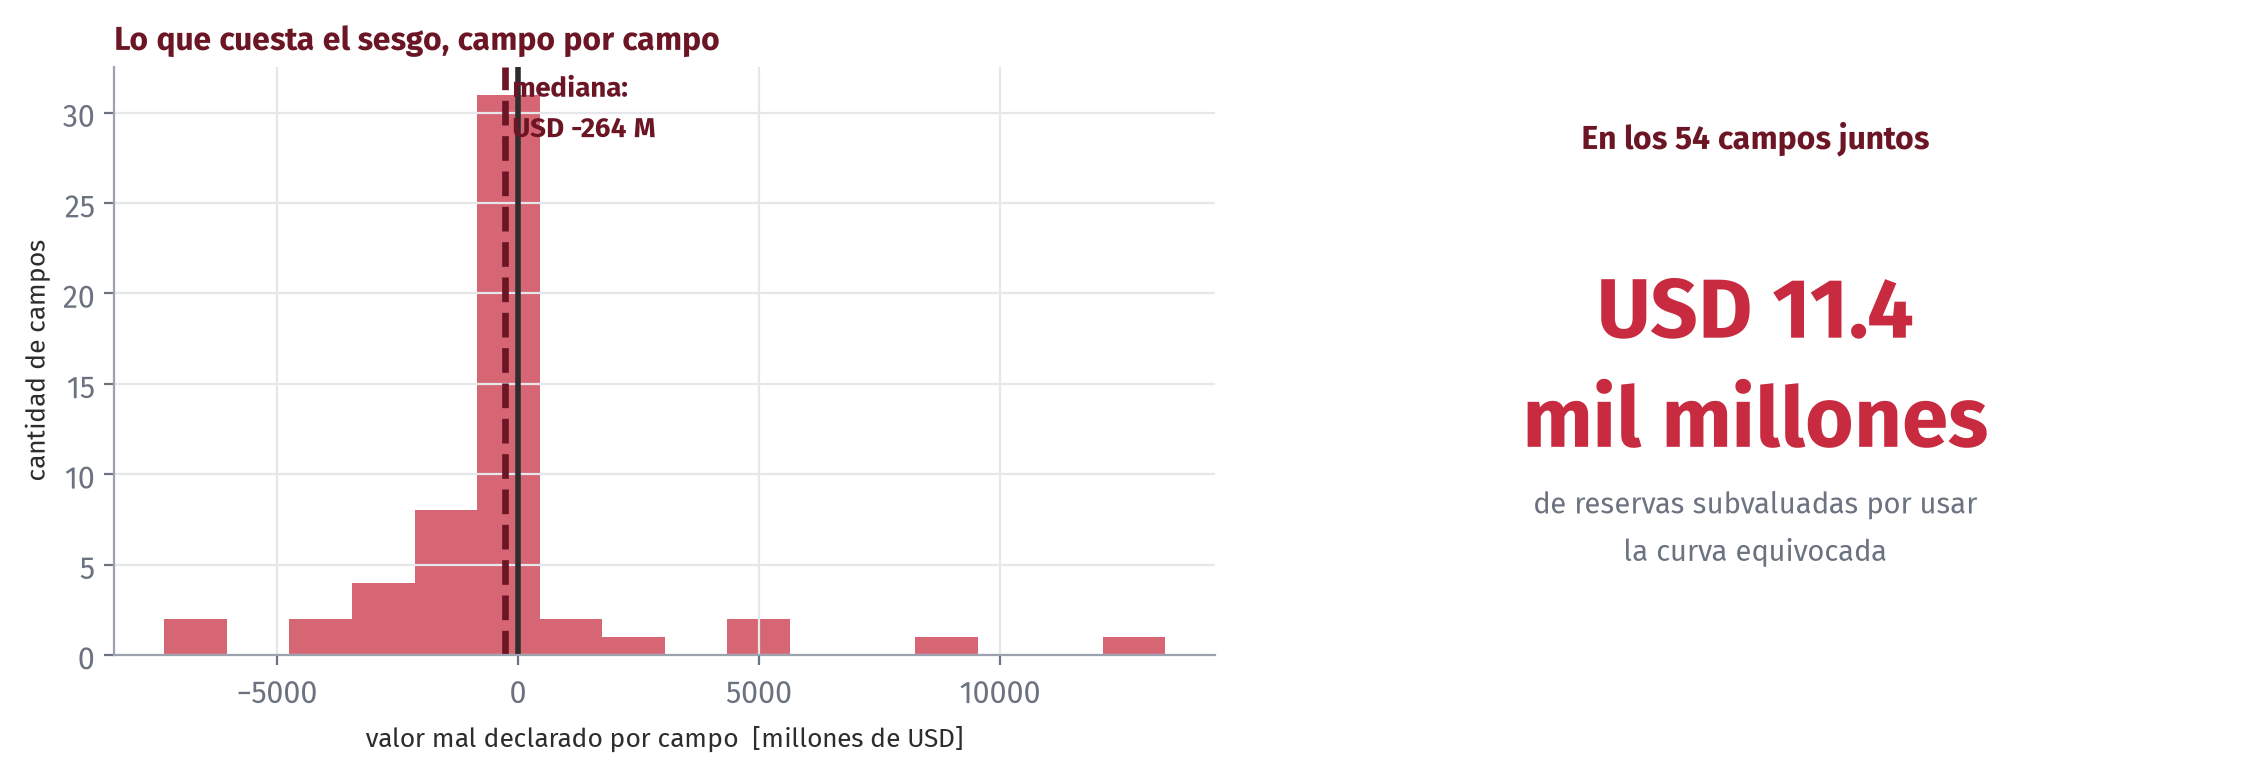
\includegraphics[height=0.54\textheight]{fig_dolares.png}
  \end{center}
  \vspace{-2pt}
  {\footnotesize\color{textMuted}
   Un 7 \% suena a nada. En un campo mediano son \textbf{264 millones de
   dólares} de reservas que no se declaran. Y como el sesgo va siempre para
   el mismo lado, en la cartera \textbf{no se compensa: se suma}.}
\end{frame}

\begin{frame}[shrink=24]{Qué Cambia una Decisión, y Qué No}
  \vspace{-4pt}
  {\small\color{arcaDark}\bfseries
   Tres números salieron de esta clase. Solo dos mueven una decisión.}
  \vspace{8pt}
  {\footnotesize
  \renewcommand{\arraystretch}{1.4}
  \begin{tabular}{@{}p{4.5cm}p{4.3cm}p{5.8cm}@{}}
    \toprule
    {\color{arcaDark}\bfseries el número} &
    {\color{arcaDark}\bfseries cuánto vale} &
    {\color{arcaDark}\bfseries qué decisión mueve} \\
    \midrule
    El sesgo de la exponencial &
      {\color{arcaRed}\bfseries USD 264 M} por campo &
      Cuántas reservas se declaran. Afecta el valor de la compañía \\
    La curva y su freno &
      {\color{arcaRed}\bfseries 19 vs 54 años} de vida &
      Cuándo se provisiona el abandono y cuándo se cierra \\
    \rowcolor{arcaGray}
    El ajuste fino de \emph{qi} &
      centavos por barril &
      {\color{textMuted}Ninguna. Y es en lo que más tiempo se gasta} \\
    \bottomrule
  \end{tabular}}
  \vspace{9pt}

  \begin{tcolorbox}[colback=arcaGray, colframe=arcaDark, boxrule=0pt, leftrule=3pt,
    arc=3pt, left=8pt, right=8pt, top=6pt, bottom=6pt]
    {\footnotesize\color{textMuted}
     La lección práctica: antes de afinar un parámetro, pregúntense
     \textbf{cuántos dólares mueve}. Si la respuesta es «no sé», ese no es
     el parámetro que hay que afinar.}
  \end{tcolorbox}
\end{frame}

% ═════════════════════════════════════════════════════════════════════════════
\sectionframe{Cuando el Número No Alcanza}{Ninguno acierta. Y eso, medido, es el resultado de la clase \\[6pt] \normalsize 80 -- 100 min}
% ═════════════════════════════════════════════════════════════════════════════

\begin{frame}[shrink=6]{El Marcador de los 54 Campos}
  \vspace{-6pt}
  \begin{center}
    
\includegraphics[height=0.58\textheight]{fig_marcador.png}
  \end{center}
  \vspace{-2pt}
  {\footnotesize\color{arcaDark}
   La hiperbólica \textbf{se ganó su lugar}: baja el error típico de 11 a
   10 \%, mata el sesgo (--7 \% $\rightarrow$ +1 \%) y baja el peor caso de
   41 \% a \textbf{29 \%}. Pero sigue errando un 10 \%.}
\end{frame}

\begin{frame}[shrink=16]{La Pregunta Incómoda}
  \vspace{6pt}
  \begin{tcolorbox}[colback=arcaGray, colframe=arcaRed, boxrule=0pt, leftrule=4pt,
    arc=3pt, left=10pt, right=10pt, top=8pt, bottom=8pt]
    {\large\color{arcaDark}\bfseries
     Si el mejor método disponible se equivoca un 10 \% ---
     y en el peor campo, un 29 \% ---\\[4pt]
     ¿por qué entregamos \emph{un} número?}
  \end{tcolorbox}
  \vspace{9pt}
  {\footnotesize\color{textMuted}
  \begin{itemize}\setlength{\itemsep}{5pt}
    \item[{\color{arcaRed}\scriptsize\faArrowRight}]
      Un número solo \textbf{esconde} exactamente la información que el que
      decide necesita: cuánto puede moverse.
    \item[{\color{arcaRed}\scriptsize\faArrowRight}]
      Y encima invita a discutir la coma. Dos ingenieros pueden pelearse una
      tarde entera por 11{,}4 contra 13{,}0 millones de barriles --- cuando el
      método entero tiene un margen de 10 \%.
    \item[{\color{codeGreen}\scriptsize\faCheck}]
      La industria ya tiene un lenguaje para esto y ustedes lo escucharon
      mil veces: \textbf{P10, P50, P90}. Lo que casi nunca se hace es
      \textbf{comprobar si esos números dicen la verdad}.
  \end{itemize}}
  \vspace{6pt}
  {\scriptsize\color{arcaDark}\itshape
   Eso es lo que vamos a hacer en los próximos veinte minutos, y es la parte
   de la clase que no van a encontrar en un curso de DCA.}
\end{frame}

\begin{frame}[shrink=24]{Qué Significan P10, P50 y P90}
  \vspace{-4pt}
  {\small\color{arcaDark}\bfseries
   Un percentil es una promesa sobre con qué frecuencia uno se equivoca.}
  \vspace{6pt}
  {\footnotesize
  \renewcommand{\arraystretch}{1.35}
  \begin{tabular}{@{}p{1.6cm}p{5.3cm}p{7.6cm}@{}}
    \toprule
    {\color{arcaDark}\bfseries nombre} &
    {\color{arcaDark}\bfseries qué dice} &
    {\color{arcaDark}\bfseries cómo se lee en voz alta} \\
    \midrule
    {\color{codeOrange}\bfseries P10} & El caso bajo &
      «Estoy bastante seguro de que produce \emph{al menos} esto» \\
    {\color{arcaDark}\bfseries P50} & La mitad &
      «Es igual de probable que quede por arriba o por abajo» \\
    {\color{codeOrange}\bfseries P90} & El caso alto &
      «Sería una sorpresa que produjera \emph{más} que esto» \\
    \bottomrule
  \end{tabular}}
  \vspace{9pt}

  \begin{tcolorbox}[colback=arcaGray, colframe=arcaDark, boxrule=0pt, leftrule=3pt,
    arc=3pt, left=8pt, right=8pt, top=6pt, bottom=6pt]
    {\scriptsize\color{arcaDark}\bfseries\faBalanceScale\hspace{4pt}LA PROMESA, DICHA CON PRECISIÓN}\\[4pt]
    {\scriptsize\color{textMuted}
     Una banda de P10 a P90 promete que \textbf{8 de cada 10 veces la
     realidad cae adentro}. Es \emph{verificable} --- y casi nadie la
     verifica, porque hacen falta muchos casos ya terminados. Tenemos 54.}
  \end{tcolorbox}
\end{frame}

\begin{frame}[shrink=16]{De Dónde Sale la Banda: la Experiencia Ajena}
  \vspace{-4pt}
  {\small\color{arcaDark}\bfseries
   Y acá está la idea de la clase, que es de sentido común antes que de
   matemática.}
  \vspace{7pt}
  {\footnotesize\color{textMuted}
  Un campo nuevo no es el primer campo del mundo. Hay \textbf{53 campos} que
  ya recorrieron el camino completo. Entonces, en vez de preguntarle a la
  fórmula, preguntémosle a ellos:
  \vspace{6pt}
  \begin{enumerate}\setlength{\itemsep}{4pt}
    \item Para cada campo terminado, miramos cuánto produjo en sus primeros
          5 años, y cuánto terminó produciendo en 12.
    \item La división de esos dos números es un \textbf{multiplicador}. Por
          ejemplo, 1{,}5 quiere decir «terminó produciendo una vez y media lo
          de sus primeros cinco años».
    \item Con 53 multiplicadores tenemos una \textbf{distribución}, no un
          número. Y de ahí salen el P10, el P50 y el P90.
  \end{enumerate}}
  \vspace{7pt}
  \begin{tcolorbox}[colback=arcaGray, colframe=arcaRed, boxrule=0pt, leftrule=3pt,
    arc=3pt, left=8pt, right=8pt, top=5pt, bottom=5pt]
    {\scriptsize\color{arcaRed}\bfseries\faExclamationTriangle\hspace{4pt}LA REGLA QUE NO SE NEGOCIA}\\[4pt]
    {\scriptsize\color{textMuted}
     Al evaluar un campo, ese campo \textbf{queda fuera} del cálculo de los
     análogos. Si se deja adentro, se está usando su propio futuro para
     predecir su futuro. Es la misma trampa del \texttt{GroupKFold} de la
     Clase 2, con otro disfraz.}
  \end{tcolorbox}
\end{frame}

\begin{frame}[shrink=6]{Los Análogos, en Dos Figuras}
  \vspace{-6pt}
  \begin{center}
    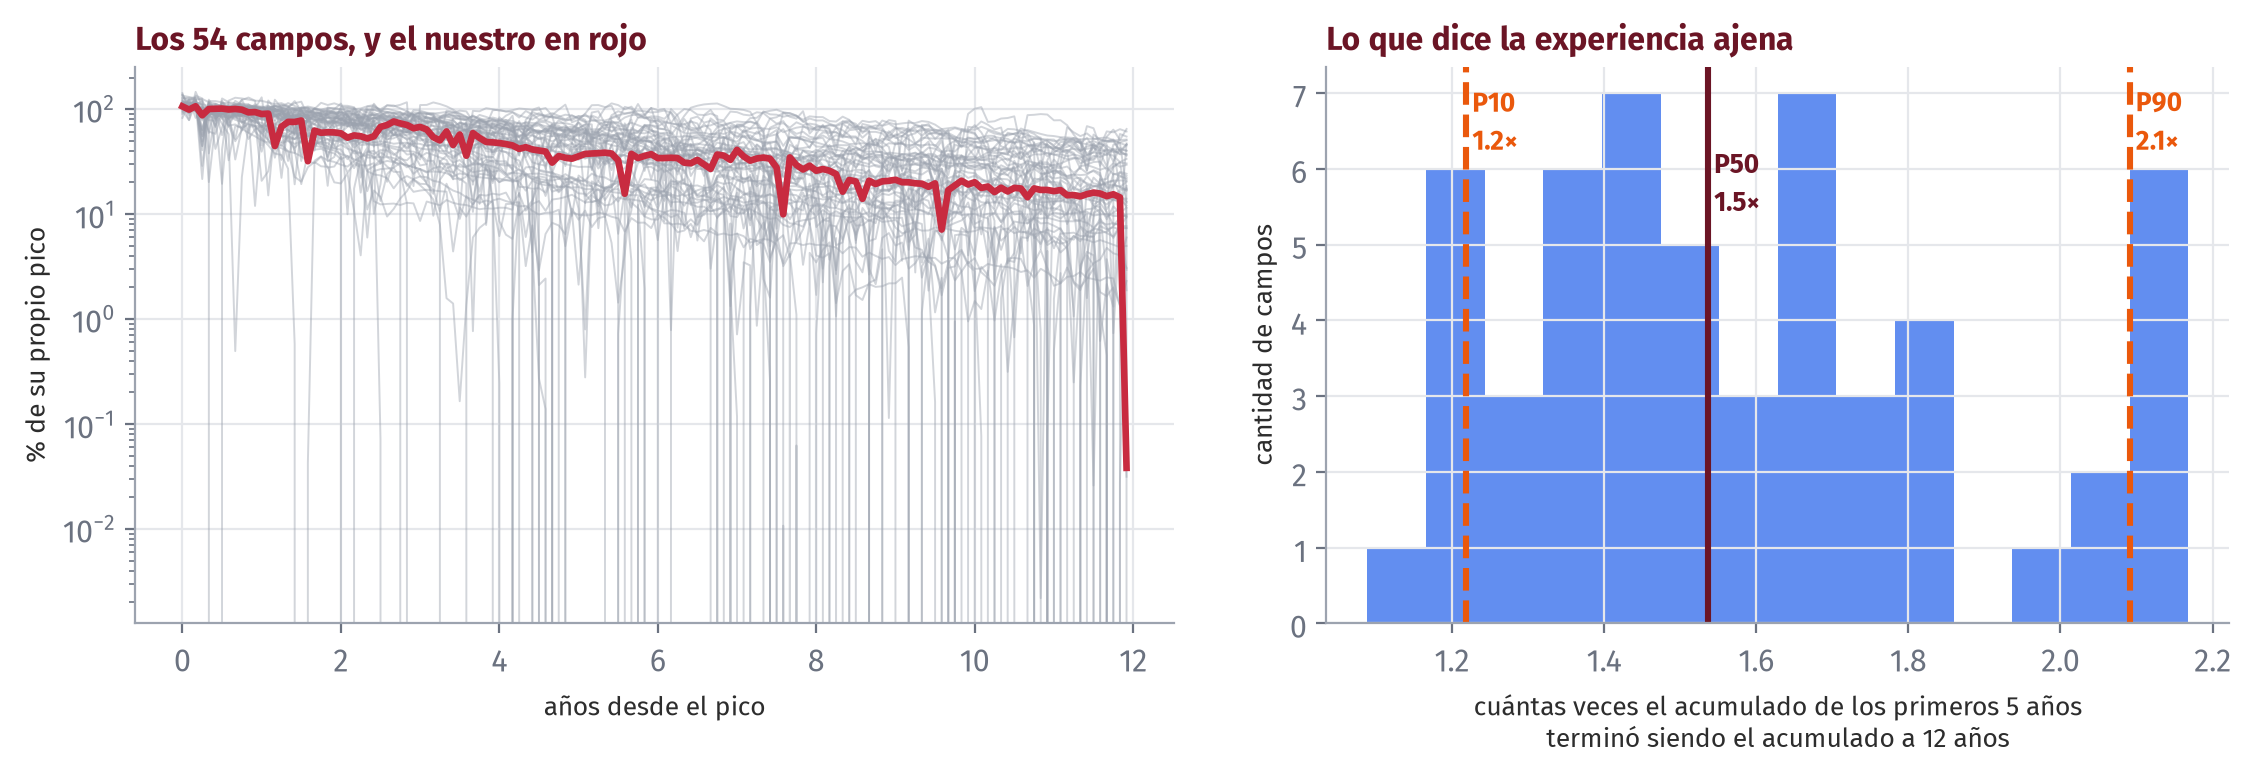
\includegraphics[height=0.56\textheight]{fig_analogos.png}
  \end{center}
  \vspace{-2pt}
  {\footnotesize\color{textMuted}
   El multiplicador va de \textbf{1{,}22$\times$} (P10) a \textbf{2{,}09$\times$}
   (P90), con mediana \textbf{1{,}54$\times$}. Esa dispersión no es ruido:
   es cuánta variedad real hay entre campos, y es exactamente lo que un
   número solo tapa.}
\end{frame}

\begin{frame}[shrink=6]{Las Tres Respuestas, y el Resultado}
  \vspace{-6pt}
  \begin{center}
    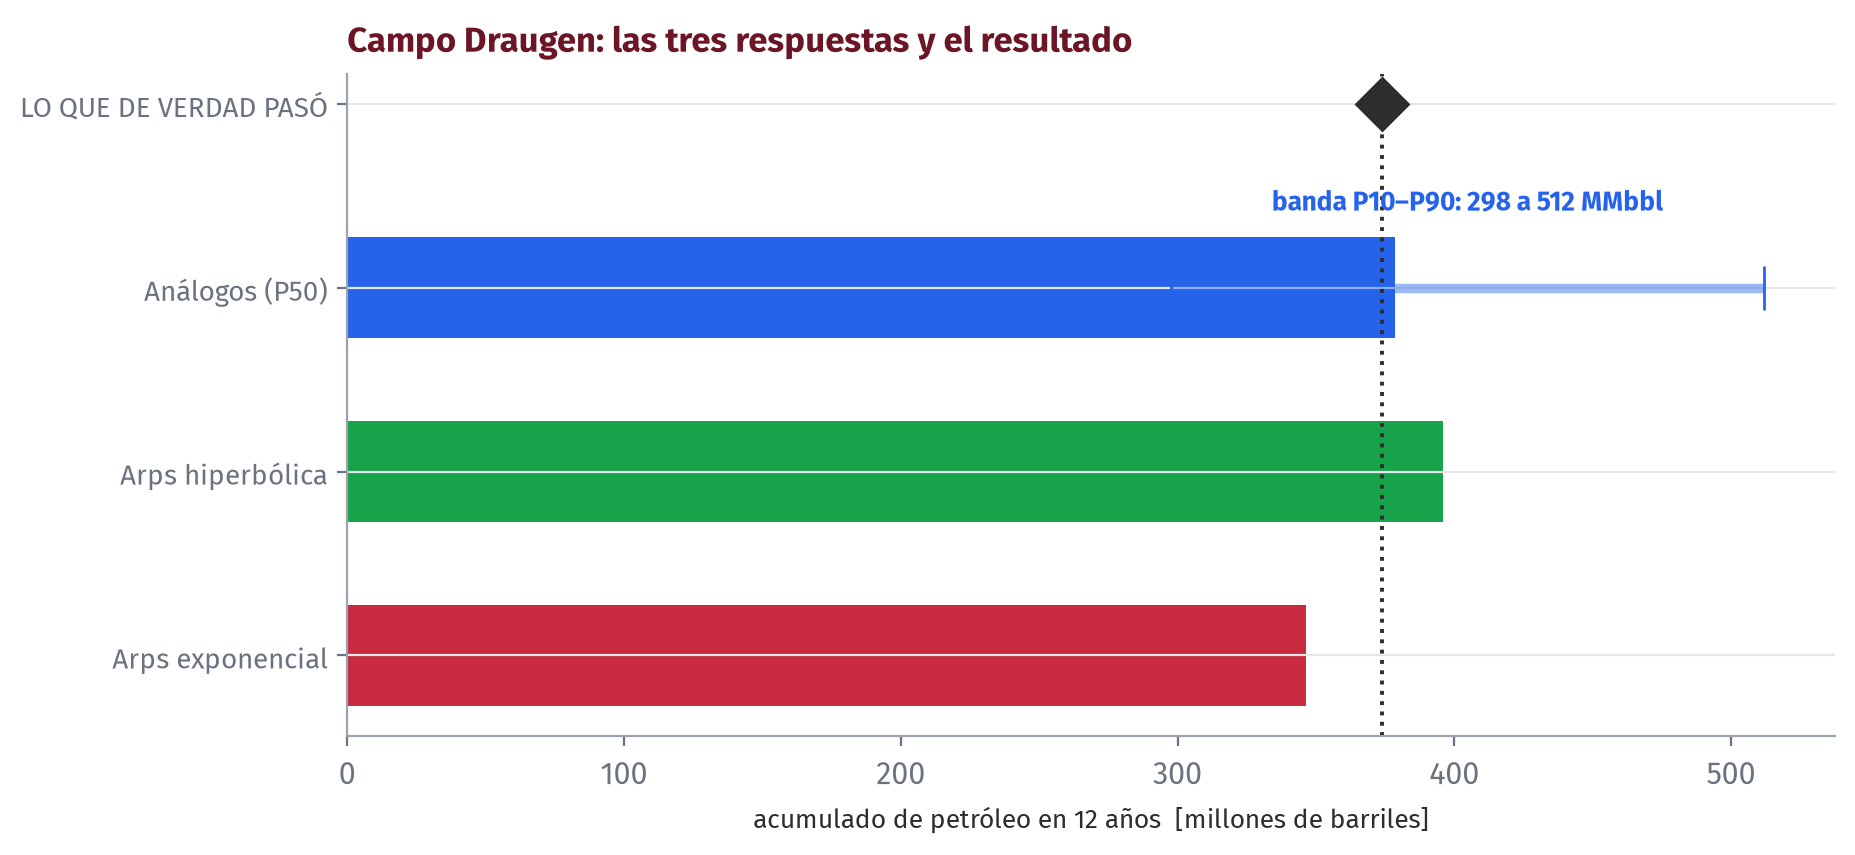
\includegraphics[height=0.54\textheight]{fig_banda.png}
  \end{center}
  \vspace{-4pt}
  {\footnotesize\color{arcaDark}
   Draugen produjo \textbf{373{,}9 millones de barriles}. La exponencial dijo
   346{,}6 (--7 \%), la hiperbólica 395{,}8 (+6 \%), los análogos 378{,}5
   (+1 \%). Y la banda de \textbf{298 a 512 lo contuvo}.}
\end{frame}

\begin{frame}[shrink=8]{Pero un Campo No Prueba Nada}
  \vspace{-4pt}
  {\small\color{arcaDark}\bfseries
   Que la banda haya acertado en Draugen puede ser suerte. La pregunta seria
   es otra.}
  \vspace{9pt}
  \begin{columns}[T]
    \begin{column}{0.49\textwidth}
      \begin{tcolorbox}[colback=arcaGray, colframe=arcaRed, boxrule=0pt, leftrule=3pt,
        arc=3pt, left=6pt, right=6pt, top=5pt, bottom=5pt]
        {\scriptsize\color{arcaRed}\bfseries\faBan\hspace{4pt}LA PREGUNTA FÁCIL}\\[4pt]
        {\scriptsize\color{textMuted}
         \textit{«¿La banda contuvo el resultado?»}\\[4pt]
         Con un solo campo, siempre se puede contestar que sí ---
         basta con hacer la banda más ancha.}
      \end{tcolorbox}
    \end{column}
    \begin{column}{0.49\textwidth}
      \begin{tcolorbox}[colback=arcaGray, colframe=codeGreen, boxrule=0pt, leftrule=3pt,
        arc=3pt, left=6pt, right=6pt, top=5pt, bottom=5pt]
        {\scriptsize\color{codeGreen}\bfseries\faCheck\hspace{4pt}LA PREGUNTA SERIA}\\[4pt]
        {\scriptsize\color{textMuted}
         \textit{«Cuando prometo 80 \%, ¿acierto el 80 \% de las veces?»}\\[4pt]
         Ni más ni menos. Una banda que acierta el 100 \% es tan
         \textbf{inútil} como una que acierta el 40 \%: la primera es tan
         ancha que no dice nada.}
      \end{tcolorbox}
    \end{column}
  \end{columns}
  \vspace{9pt}
  {\footnotesize\color{arcaDark}
   A eso se le llama \textbf{calibración}, y es lo único que distingue un
   intervalo honesto de un adorno. Se mide repitiendo el ejercicio en los
   54 campos, dejando cada uno afuera por turno.}
\end{frame}

\begin{frame}[shrink=6]{¿Cumple lo que Promete?}
  \vspace{-6pt}
  \begin{center}
    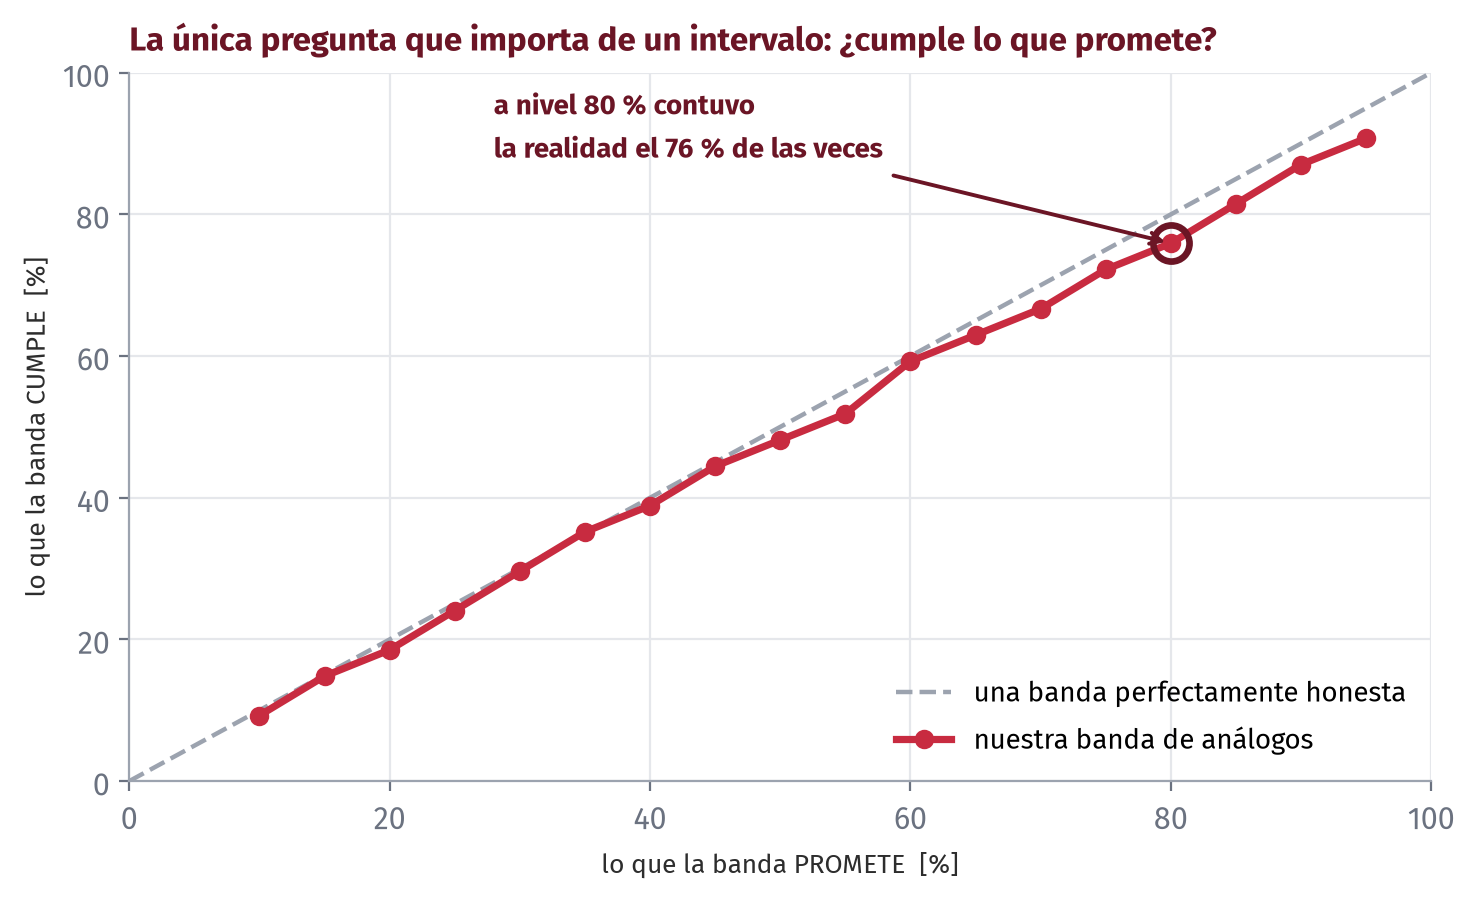
\includegraphics[height=0.56\textheight]{fig_calibracion.png}
  \end{center}
  \vspace{-4pt}
  {\footnotesize\color{arcaDark}
   La curva roja sigue a la diagonal en todo el rango. En 41 de 54 campos
   ---\textbf{el 76 \%}--- la realidad cayó dentro de la banda que prometía
   80 \%.}
\end{frame}

\begin{frame}[shrink=16]{Cómo Reportarlo al que Decide}
  \vspace{-4pt}
  \begin{columns}[T]
    \begin{column}{0.48\textwidth}
      \begin{tcolorbox}[colback=arcaGray, colframe=arcaRed, boxrule=0pt, leftrule=3pt,
        arc=3pt, left=6pt, right=6pt, top=5pt, bottom=5pt]
        {\scriptsize\color{arcaRed}\bfseries\faBan\hspace{4pt}ASÍ NO}\\[5pt]
        {\scriptsize\color{textMuted}\itshape
         «Ajustamos una declinación hiperbólica de Arps con b = 0{,}91 y
         obtuvimos un EUR a 12 años de 395{,}8 MMbbl.»}\\[5pt]
        {\scriptsize\color{textMuted}
         Suena preciso y no lo es. No dice cuánto puede moverse, ni con qué
         confianza, ni qué pasa si se mueve.}
      \end{tcolorbox}
    \end{column}
    \begin{column}{0.48\textwidth}
      \begin{tcolorbox}[colback=arcaGray, colframe=codeGreen, boxrule=0pt, leftrule=3pt,
        arc=3pt, left=6pt, right=6pt, top=5pt, bottom=5pt]
        {\scriptsize\color{codeGreen}\bfseries\faCheck\hspace{4pt}ASÍ SÍ}\\[5pt]
        {\scriptsize\color{textMuted}\itshape
         «Lo más probable son \textbf{378 millones} de barriles en 12 años, y
         con 8 de cada 10 de confianza está entre \textbf{298 y 512}.\\[4pt]
         Ese rango lo verificamos contra 54 campos que ya terminaron: la
         banda acertó el \textbf{76 \%} de las veces, cuando prometía 80 \%.
         Es honesta.\\[4pt]
         Si el proyecto no cierra con 298, no cierra.»}
      \end{tcolorbox}
    \end{column}
  \end{columns}
  \vspace{7pt}
  {\footnotesize\color{arcaDark}\itshape
   La segunda versión se puede \textbf{decidir}. Y además dice de dónde sale
   la confianza --- que es lo que un auditor de reservas va a preguntar.}
\end{frame}

\begin{frame}[shrink=8]{Lo que Esto NO Autoriza a Decir}
  \vspace{-4pt}
  {\small\color{arcaDark}\bfseries
   Una clase honesta también dice dónde se rompe su propio método.}
  \vspace{8pt}
  {\footnotesize\color{textMuted}
  \begin{itemize}\setlength{\itemsep}{6pt}
    \item[{\color{arcaRed}\scriptsize\faTimes}]
      \textbf{No sirve para un campo sin análogos.} Si el campo es de un tipo
      que no está entre los 54 --- otra roca, otro fluido, otra tecnología ---
      la banda no aplica. La calibración se hereda del grupo, no del campo.
    \item[{\color{arcaRed}\scriptsize\faTimes}]
      \textbf{No incluye decisiones futuras.} Si mañana se aprueba una
      campaña de perforación o un proyecto de recuperación mejorada, la
      producción cambia por una razón que ningún análogo puede anticipar.
    \item[{\color{arcaRed}\scriptsize\faTimes}]
      \textbf{54 campos son pocos.} El P10 y el P90 se estiman con las colas
      de la muestra, que es donde menos datos hay. Con 54 casos, ese 76 \%
      tiene su propia incertidumbre.
    \item[{\color{codeGreen}\scriptsize\faCheck}]
      \textbf{Sí sirve} para lo que se pidió: poner un rango defendible y
      auditado alrededor de un número que hoy se firma solo.
  \end{itemize}}
\end{frame}

% ═════════════════════════════════════════════════════════════════════════════
\sectionframe{Su Turno}{Un campo, de punta a punta \\[6pt] \normalsize 100 -- 118 min}
% ═════════════════════════════════════════════════════════════════════════════

\begin{frame}[shrink=16]{Su Turno: Firmen un Número \hfill {\normalsize\color{arcaRed}\faClock\hspace{4pt}25 min}}
  \vspace{-4pt}
  \begin{tcolorbox}[colback=arcaGray, colframe=arcaDark, boxrule=0pt, leftrule=3pt,
    arc=3pt, left=8pt, right=8pt, top=5pt, bottom=5pt]
    {\footnotesize\color{arcaDark}\itshape
     Les toca el campo \textbf{GULLFAKS}: 32 años de historia después del
     pico y un pico de 569 mil barriles por día. Es de los grandes.}
  \end{tcolorbox}
  \vspace{7pt}
  {\footnotesize\color{textMuted}
  \begin{enumerate}\setlength{\itemsep}{4pt}
    \item Corran la celda ya escrita: les arma la serie de Gullfaks desde el
          pico y les tapa todo lo posterior al año 5. \textbf{El primer paso
          está resuelto.}
    \item Ajusten la \textbf{exponencial}. ¿Cuál es su D anual? ¿Es un campo
          que declina rápido o lento comparado con la mediana de 18 \%?
    \item Ajusten la \textbf{hiperbólica}. ¿Qué b les dio? ¿Este campo tiene
          cola o no?
    \item Construyan la \textbf{banda de análogos} --- acordándose de sacar a
          Gullfaks del grupo.
    \item Destapen y comparen. ¿Cuál de los tres estuvo más cerca?
          ¿La banda contuvo la realidad?
    \item {\color{arcaDark}\bfseries Pregunta de negocio:} escriban
          \textbf{dos frases} para el comité de reservas. La primera dice el
          número que firman y su rango. La segunda dice \textbf{qué haría
          falta para que ese rango se angoste} --- porque eso es lo que van a
          preguntar.
  \end{enumerate}}
\end{frame}

% ═════════════════════════════════════════════════════════════════════════════
\sectionframe{Cierre}{}
% ═════════════════════════════════════════════════════════════════════════════

\begin{frame}[shrink=10]{Lo Que Aprendimos Hoy}
  \vspace{-4pt}
  \begin{columns}[T]
    \begin{column}{0.48\textwidth}
      {\small\color{arcaDark}\bfseries\faLightbulb[regular]\hspace{5pt}Conceptos:}
      \vspace{4pt}
      {\footnotesize\color{textMuted}
      \begin{itemize}\setlength{\itemsep}{3pt}
        \item[{\color{codeGreen}\scriptsize\faCheck}]
          \textbf{Arps} (1945): exponencial, hiperbólica y armónica
        \item[{\color{codeGreen}\scriptsize\faCheck}]
          \textbf{D} es la tasa de declinación; \textbf{b} es la cola
        \item[{\color{codeGreen}\scriptsize\faCheck}]
          \textbf{Error} y \textbf{sesgo} no son lo mismo, y el sesgo
          no se compensa
        \item[{\color{codeGreen}\scriptsize\faCheck}]
          \textbf{P10 / P50 / P90} es una promesa, y las promesas se auditan
        \item[{\color{codeGreen}\scriptsize\faCheck}]
          \textbf{Calibración}: la única prueba de que un intervalo es honesto
      \end{itemize}}
    \end{column}
    \begin{column}{0.48\textwidth}
      {\small\color{arcaDark}\bfseries\faTools\hspace{5pt}Herramientas:}
      \vspace{4pt}
      {\footnotesize\color{textMuted}
      \begin{itemize}\setlength{\itemsep}{3pt}
        \item[{\color{arcaRed}\scriptsize\faArrowRight}]
          \texttt{np.polyfit} sobre \texttt{np.log} --- el ajuste exponencial
        \item[{\color{arcaRed}\scriptsize\faArrowRight}]
          \texttt{scipy.optimize.curve\_fit} con \texttt{bounds}
        \item[{\color{arcaRed}\scriptsize\faArrowRight}]
          \texttt{.quantile([0.1, 0.5, 0.9])} --- los percentiles
        \item[{\color{arcaRed}\scriptsize\faArrowRight}]
          Validación \textbf{dejando uno afuera} (\emph{leave-one-out})
      \end{itemize}}
      \vspace{6pt}
      \begin{tcolorbox}[colback=arcaGray, colframe=arcaRed, boxrule=0pt, leftrule=3pt,
        arc=3pt, left=6pt, right=6pt, top=4pt, bottom=4pt]
        {\scriptsize\color{arcaRed}\bfseries EL NÚMERO DEL DÍA}\\[3pt]
        {\scriptsize\color{textMuted}
         \textbf{76 \%.} Lo que cumplió una banda que prometía 80 \%.
         Casi nadie mide esto, y es lo único que la valida.}
      \end{tcolorbox}
    \end{column}
  \end{columns}
\end{frame}

\begin{frame}[shrink=8]{Si Se Llevan Una Sola Cosa}
  \vspace{6pt}
  \begin{tcolorbox}[colback=arcaGray, colframe=arcaRed, boxrule=0pt, leftrule=4pt,
    arc=3pt, left=10pt, right=10pt, top=9pt, bottom=9pt]
    {\large\color{arcaDark}\bfseries
     Un pronóstico sin banda no es un pronóstico: es una opinión con
     decimales.}\\[7pt]
    {\footnotesize\color{textMuted}
     Y una banda sin calibrar tampoco vale: cualquiera puede inventar un
     rango lo bastante ancho como para no equivocarse nunca.\\[6pt]
     Lo que convierte un rango en una \textbf{entrega de ingeniería} es
     haberlo puesto a prueba contra casos que ya terminaron, y poder decir
     cuántas veces acertó.}
  \end{tcolorbox}
  \vspace{8pt}
  {\footnotesize\color{arcaDark}\itshape
   Fíjense que esto no dependió del algoritmo. Dependió de tener 53 campos
   que ya habían recorrido el camino --- y de acordarse de sacar el nuestro
   del grupo.}
\end{frame}

\begin{frame}[shrink=8]{Lo Que Sigue}
  \vspace{4pt}
  {\footnotesize\color{textMuted}
  \begin{itemize}\setlength{\itemsep}{9pt}
    \item[{\color{arcaRed}\faArrowCircleRight}]
      \textbf{Clase 4 --- El agua y el gas.} La segunda causa de la
      declinación, de frente: corte de agua, \textbf{WOR} y \textbf{GOR}, y
      cuándo llega el agua a un pozo (\emph{breakthrough}). El agua es el
      costo número uno de un campo maduro.
    \item[{\color{arcaRed}\faArrowCircleRight}]
      \textbf{Clase 5 --- El equipo.} Bombas \textbf{ESP} y levantamiento
      artificial: el método de detección de la Clase 2, ahora sobre el equipo
      que más se rompe y más caro cuesta reparar.
  \end{itemize}}
  \vspace{9pt}
  \begin{tcolorbox}[colback=arcaGray, colframe=codeGreen, boxrule=0pt, leftrule=3pt,
    arc=3pt, left=8pt, right=8pt, top=5pt, bottom=5pt]
    {\scriptsize\color{codeGreen}\bfseries\faCheck\hspace{4pt}DEUDA SALDADA}\\[4pt]
    {\scriptsize\color{textMuted}
     En la Clase 1 ajustamos una recta sobre el logaritmo de la producción y
     dijimos que después le poníamos nombre. Hoy se llamó
     \textbf{declinación exponencial de Arps}, se le midió el defecto, y se
     la reemplazó por algo mejor. Queda cerrada.}
  \end{tcolorbox}
\end{frame}

\begin{frame}[shrink=10]{Datos y Referencias}
  \vspace{4pt}
  {\footnotesize\color{textMuted}
  \begin{itemize}\setlength{\itemsep}{6pt}
    \item[{\color{arcaRed}\scriptsize\faDatabase}]
      \textbf{Sokkeldirektoratet} (Norwegian Offshore Directorate) ---
      \emph{Production figures, monthly by field}. Datos abiertos.
      \texttt{factpages.sodir.no}\\
      Es la misma fuente del campo Volve que usamos en el Módulo 1 y en la
      Clase 1.
    \item[{\color{arcaRed}\scriptsize\faBook}]
      \textbf{Arps, J. J. (1945).} \textit{Analysis of Decline Curves}.
      Transactions of the AIME, 160(01), 228--247.
    \item[{\color{arcaRed}\scriptsize\faFileCode}]
      El subconjunto se arma con \texttt{modulo5-clase3/preparar\_datos.py};
      las figuras y \textbf{todas} las cifras de estas láminas salen de
      \texttt{figuras.py}. Nada está escrito a mano.
  \end{itemize}}
  \vspace{8pt}
  {\scriptsize\color{arcaDark}\itshape
   Como siempre: clonan el repositorio, corren los dos scripts, y tiene que
   dar exactamente lo mismo. Si no da, es un error nuestro y queremos saberlo.}
\end{frame}

% ── GRACIAS ──────────────────────────────────────────────────────────────────
\begingroup
\setbeamertemplate{headline}{}
\setbeamertemplate{footline}{}
\setbeamertemplate{navigation symbols}{}
\begin{frame}[plain, noframenumbering]
  \begin{tikzpicture}[remember picture, overlay]
    \fill[arcaDark] (current page.south west) rectangle (current page.north east);
    \node[anchor=center, text=white, font=\Huge\bfseries]
      at ([yshift=1.5cm]current page.center) {¡Gracias!};
    \node[anchor=center, text=white!80, font=\large, text width=10cm, align=center]
      at ([yshift=0.2cm]current page.center)
      {Carlos Enrique Mosquera Trujillo};
    \node[anchor=center, text=white!60, font=\normalsize, text width=10cm, align=center]
      at ([yshift=-0.6cm]current page.center)
      {\faEnvelope\hspace{6pt}cmosquerat@unal.edu.co};
    \node[anchor=center, text=white!60, font=\normalsize, text width=11cm, align=center]
      at ([yshift=-1.3cm]current page.center)
      {Machine Learning for Petroleum Engineers Using Python};
    \node[anchor=center, text=white!40, font=\small]
      at ([yshift=-2.0cm]current page.center)
      {Módulo 5 · Clase 3 \quad$\cdot$\quad SLB Ecuador \quad$\cdot$\quad UDLA \quad$\cdot$\quad 2026};
  \end{tikzpicture}
\end{frame}
\endgroup

\end{document}
